\RequirePackage{silence} % :-\
    \WarningFilter{scrbook}{Usage of package `titlesec'}
    \WarningFilter{titlesec}{Non standard sectioning command detected}
\documentclass[11pt,paper=b5,footinclude,headinclude]{scrbook} % KOMA-Script book
\usepackage[T1]{fontenc}
\usepackage[style=arsclassica, parts=false, eulermath=false, palatino=true, eulerchapternumbers=true]{classicthesis}

\usepackage[Export]{adjustbox}


%\documentclass[11pt,a5paper,footinclude,headinclude]{scrbook} % KOMA-Script book

\usepackage{xspace,xcolor,afterpage}
\usepackage{url}
\usepackage{enumitem}
\usepackage{comment}
\usepackage{graphicx}
\usepackage{amsfonts,amsmath,amssymb,amsthm}
\usepackage{graphics}
\usepackage{color}
\usepackage{fullpage}
\usepackage{makecell}
\usepackage{answers}
%\usepackage{times}
%\usepackage{txfonts}
\def\P {{\cal P}}
\def\ali {{~\vee~}}
\def\inn {{~\wedge~}}
\def\sledi {{~\Rightarrow~}}
\def\brez {{\,\setminus\,}}
\def\cee {{~\Leftrightarrow~}}
\def\zgled{\paragraph{Example:}}
\def\kz{{\hfill{\S}}}% konec zgleda
\newenvironment{example}{\paragraph{Example:}}{\hfill \S}

\theoremstyle{remark}
\newtheorem*{remark}{Remark}
\newtheorem*{lemma}{Lemma}
\newtheorem*{corollary}{Corollary}
\theoremstyle{definition} %theorem
\newtheorem*{definition}{Definition}
\theoremstyle{theorem} %theorem
\newtheorem*{theorem}{Theorem}
\newtheorem*{proposition}{Proposition}


\newtheorem{ex}{Exercise\hypertarget{sol:\theex}}[chapter]
% \newtheorem{ex}{\hyperlink{ex:\theex}{Vaja}\hypertarget{sol:\theex}}[chapter]
\Newassociation{sol}{answer}{ans}
\renewenvironment{answer}[1]
{\par\bigskip\noindent{\bfseries \hypertarget{ex:#1}{}\hyperlink{sol:#1}{Answer for exercise #1:}}\quad}
{\par\bigskip}

%vars
\newcommand{\myTitle}{Theoretical Computer Science\xspace}
\newcommand{\mySubtitle}{Discrete Structures for Computer Science Students \xspace} 				%dodaj podnaslov if needed
\newcommand{\myName}{UP FAMNIT \xspace}
\newcommand{\myPublisher}{Matjaž Krnc}
\newcommand{\myMonth}{Fall}
\newcommand{\myYear}{2024}
\newcommand{\verzija}{Version 0.1\xspace}
\newcommand{\shortAuthors}{M. Krnc}
\newcommand{\myAuthors}{Matjaž Krnc}
\newcommand{\myISBN}{978-961-XXX-XXX-X }
\newcommand{\myRepo}{\url{https://github.com/mkrnc/TOR1-vaje---TCS1-exercises.git}}


\begin{document}
\input{Titlepage}
\input{en/cip}
\newpage
\section*{Preface}
   

Those notes are supposed to be parsed together with explanations from the lectures.
Any questions or found errors should be 
addressed to \url{matjaz.krnc@upr.si}, or 
raised as an issue in our public repository 
\begin{center}
    \myRepo.    
\end{center}


Among most notable student contributors are:


\input{en/kolofon}

\tableofcontents
\Opensolutionfile{ans}[ans1] 

\chapter{Mathematical Logic}
\section{Basic exercises}
\begin{ex}
    The following two propositions are given:
A: "It is cold outside."
B: "It is raining outside."

Write the following compound propositions in natural language:
\begin{itemize}
    \item (a) $\neg A$
    \item (b) $A \land B$
    \item (c) $A \lor B$
    \item (d) $B \lor \neg A$
\end{itemize}
\end{ex}





\begin{ex}     
The following two propositions are given:
A: "Janez is rich."
B: "Janez is happy."

Write the following propositions symbolically:
\begin{itemize}
    \item (a) If Janez is rich, then he is unhappy.
    \item (b) Janez is neither happy nor rich.
    \item (c) Janez is happy only if he is poor.
    \item (d) Janez is poor if and only if he is unhappy.
\end{itemize}

\end{ex} \begin{ex} 
Find the truth tables for the examples from the previous task.


\end{ex} 
\begin{ex}
Is the following reasoning correct?

\begin{itemize}
    \item Premise 1: "I think, therefore I am."
    \item Premise 2: "I think, therefore I reason."
    \item Conclusion: "I am, therefore I reason."
\end{itemize}
\begin{sol}
The logical implication is:

\[
(A_1 \Rightarrow A_2) \land (A_1 \Rightarrow A_3) \Rightarrow (A_2 \Rightarrow A_3)
\]

For \( A_1(d) = 0 \), \( A_2(d) = 1 \), \( A_3(d) = 0 \), this implication is false. Therefore, the reasoning is incorrect.
\end{sol}




\end{ex} \begin{ex}
The following two propositions are given:
$A$: ``Andrej speaks French.'' and $B$: ``Andrej speaks Danish.''
Write the following compound propositions in natural language:

(a) $A\ali B$

(b) $A\inn B$

(c) $A\inn \neg B$

(d) $\neg A\ali \neg B$

(e) $\neg \neg A$

(f) $\neg (\neg A\inn \neg B)$


\end{ex} \begin{ex} \label{ex:newspapers} Given the propositions:\\
$A:$ ``John reads The New York Times.''\\
$B:$ ``John reads The Wall Street Journal.''\\
$C:$ ``John reads The Daily Mail.''\\
\\
Transcribe the following statements into symbolic propositions:
\begin{enumerate}
\item John reads The New York Times, but not The Wall Street Journal.
\item Either John reads both The New York Times and The Wall Street Journal,
or he does not read The New York Times and The Wall Street Journal.
\item It is not true that John reads The New York Times, and does not read
The Daily Mail.
\item It is not true that John reads The Daily Mail or The Wall Street Journal,
and not The New York Times.
\end{enumerate}
\end{ex} \begin{ex} Find the truth tables for the symbolic propositions from Exercise \ref{ex:newspapers}.


\end{ex} \begin{ex} For three lines $p,q,r$ we may construct also geometric propositions.
Suppose that the following is true:
\[
(p||q)\wedge(p\cap q\neq\emptyset)\wedge(q\cap r\neq\emptyset).
\]
What can you say about the lines $p,q,r$?



\end{ex}
\begin{ex} Express the propositions below with connectives $\wedge$ and $\neg$
only!
\begin{enumerate}
\item $A\vee B$
\item $A\Rightarrow B$
\item $A\Leftrightarrow B$
\end{enumerate}
\end{ex}

\section{Knights and servants (kneves)}
Knights always tell the truth, while servants always lie.



\begin{ex} 
 Artur: "It is not true that Cene is a servant."
 
Bine: "Cene is a knight or I am a knight."

Cene: "Bine is a servant."

For each of them, determine whether they are knights or servants!

% \textbf{Solut6 0$ and  $B = 1$. 

\end{ex} \begin{ex} Artur: "Cene is a servant or Bine is a servant."

Bine: "Cene is a knight and Artur is a knight."

For each of them, determine whether they are knights or servants!

% \textbf{Solution:}
\begin{sol}
    
Let us denote: $A$ – Arthur is a knight, $B$ – Bine is a knight, $C$ – Cene is a knight.

The following compound statement holds:

\[
(A \iff \neg C \lor \neg B) \land (B \iff C \land A)
\]

With the help of the truth table, we see that the statement is true only for the set $A = 1$ and $B = C = 0$.
\end{sol}

    \end{ex} \begin{ex} Let us analyze the statements made by A, B, C, and D:

\begin{itemize}
    \item A: "D is a servant and C is a servant."
    \item B: "If A and D are servants, then C is a servant."
    \item C: "If B is a servant, then A is a knight."
    \item D: "If E is a servant, then both C and B are servants."
\end{itemize}

%%solution
\begin{sol}
Let \( A \) represent "A is a knight", etc. We seek the only solution \( d \) such that the following is true:

\[
A_1 \land B_1 \land C_1 \land D_1
\]

where:
\begin{align*}
A_1 &: A \iff (\neg D \land \neg C)\\
B_1 &: B \iff (\neg A \land \neg D \Rightarrow \neg C)\\
C_1 &: C \iff (\neg B \Rightarrow A)\\
D_1 &: D \iff (\neg E \Rightarrow \neg C \land \neg B)\\
\end{align*}


Since the truth table would contain 32 rows, we solve this by analyzing cases.

\subsection*{Case 1: \( A(d) = 1 \)}

Given \( A_1 \), \( D(d) = 0 \) and \( C(d) = 0 \). Substituting into \( C_1 \) with \( A(d) = 1 \) and \( C(d) = 0 \), we get:

\[
\neg (\neg B \Rightarrow 1) \Rightarrow \neg(B \lor 1) \Rightarrow \neg 1
\]

which is a false statement. Hence, this case is not possible.

\subsection*{Case 2: \( A(d) = 0 \)}

Given \( A_1 \), either \( C(d) = 1 \) or \( D(d) = 1 \).

\subsection*{Case 2.1: \( C(d) = 1 \)}

Since \( C_1 \), \( \neg B \Rightarrow 0 \), implies \( \neg B = 0 \), hence \( B(d) = 1 \).

Substituting into \( B_1 \) with \( A(d) = 0 \), \( B(d) = 1 \), and \( C(d) = 1 \), we get:

\[
1 \land \neg D \Rightarrow 0 \Rightarrow \neg D = 0
\]

thus, \( D(d) = 1 \).

Substituting into \( D_1 \), we get:

\[
\neg E \Rightarrow 0 \land 0
\]

Hence \( E(d) = 1 \).

\subsection*{Case 2.2: \( C(d) = 0 \) and \( D(d) = 1 \)}

From \( B_1 \), we get \( B(d) = 1 \), but the statement \( C_1 \) becomes false: \( 0 \iff (0 \Rightarrow 1) \).

Thus, \( B \), \( C \), \( D \), and \( E \) are knights, while \( A \) is a servant.

\end{sol}


\end{ex}
\begin{ex} Solve the following exercises about knights and servants:
\begin{itemize}
  \item Arthur: ``It is not true that Bine is a servant."
  \item Bine: ``We are not both of the same kind.''
\end{itemize}




\end{ex} 
\begin{ex} 
Now Arthur and Bine say the following:
\begin{itemize}
 \item Arthur: ``Me and Bine are not of the same kind.''
 \item Bine: ``Exactly one of us is a knight.''
\end{itemize}


\end{ex} 
\begin{ex} Knights and servants! 
\begin{enumerate}

\item Arthur: Chloe or Bob are servants.
\item 
Bob: Cene and Arthur are knights.
\end{enumerate}
\end{ex}



\section{Canonical Forms}
     \begin{ex} Find the canonical disjunctive normal form (DNF) and the canonical conjunctive normal form (CNF) for the following propositions:
    \begin{enumerate}[label=(\roman*)]
        \item $\neg(A \land B) \Rightarrow (\neg B \Rightarrow A)$
        \item $\neg(A \lor B) \land (A \Rightarrow B)$
        \item \((A \lor \neg B) \land (B \Rightarrow A)\)
    \item \((\neg A \lor B) \Rightarrow (\neg B \lor A)\)
    \item \(\neg((A \lor B) \land (\neg A \lor \neg C))\)
    \end{enumerate}

\end{ex}
\begin{ex} For the following compound proposition find  a truth table, determine DNF, CNF and draw the corresponding circuit.
$$
(A \Rightarrow (B\Rightarrow C)) \Rightarrow ((A\Rightarrow B)\Rightarrow (A \Rightarrow C)).
$$
\end{ex}



\begin{ex}
For the following compound proposition, create a truth table, determine the DNF and CNF, and draw the corresponding circuit diagram:
\[
\neg((A \land B) \Rightarrow (\neg C \lor D)).
\]
\end{ex}

\begin{ex}
Determine if the following logical equivalences hold. Justify your answers by transforming each side into its canonical form:
\begin{itemize}
    \item[(i)] \((A \Rightarrow B) \lor (\neg A \land \neg B) \sim \neg B \Rightarrow \neg A\)
    \item[(ii)] \((A \land (B \lor C)) \Rightarrow (A \land B) \sim (\neg A \lor B)\)
\end{itemize}
\end{ex}

\begin{ex}
Prove or disprove the validity of the following compound proposition using truth tables, DNF, or CNF:
\[
(\neg A \lor B) \land (B \Rightarrow C) \sim (\neg A \lor C).
\]
\end{ex}

\begin{ex}
Simplify the following compound proposition using the laws of logic, and then find its canonical DNF and CNF:
\[
(\neg A \land (B \lor C)) \lor (A \land \neg B \land \neg C).
\]
\end{ex}

\begin{ex}
Find DNF and CNF (if they exist) for the following proposition:
\[
(A \lor B) \land (\neg A \lor C) \land (\neg B \lor \neg C).
\]
\end{ex}

\section{Switching circuits}

     \begin{ex} For the circuits in Figure \ref{fig:circuits}, find the corresponding compound propositions.\label{ex:circuits}


\begin{figure}
    \centering
    \includegraphics[width=0.26\linewidth]{img/vez1.pdf}
    \includegraphics[width=0.35\linewidth]{img/vez2.pdf}
    \includegraphics[width=0.36\linewidth]{img/vez3.pdf}
    \caption{Switching circuits for Exercise \ref{ex:circuits}.}
    \label{fig:circuits}
\end{figure}



    \end{ex} \begin{ex} For the following compound proposition, find a truth table, determine DNF, CNF, and draw the corresponding circuit.
\[
(A \Rightarrow (B \Rightarrow C)) \Rightarrow ((A \Rightarrow B) \Rightarrow (A \Rightarrow C))
\]
    \end{ex} \begin{ex} Find a compound proposition $I$ such that
\[
(A \Rightarrow (I \Rightarrow \neg B)) \Rightarrow (A \land B) \lor I
\]
is a tautology.
\end{ex}


\section{Logical Implications}

     \begin{ex} \label{ex:logical-implications}Prove the following logical equivalences:
        \begin{itemize}
            \item[(1)] $(A \Rightarrow B) \land (B \Rightarrow C) \Rightarrow (A \Rightarrow C)$
            \item[(2)] $(A \Rightarrow B) \Rightarrow ((C \Rightarrow A) \Rightarrow (C \Rightarrow B))$
            \item[(3)] $(A \Rightarrow B) \Rightarrow ((B \Rightarrow C) \Rightarrow (A \Rightarrow C))$
            \item[(4)] $(A \Rightarrow B) \Rightarrow (A \land C \Rightarrow B \land C)$
            \item[(5)] $(A \Rightarrow B) \Rightarrow (A \lor C \Rightarrow B \lor C)$
            \item[(6)] $(A \Leftrightarrow B) \land (B \Leftrightarrow C) \Rightarrow (A \Leftrightarrow C)$
            \item[(7)] $(A \Leftrightarrow B) \Rightarrow (A \Rightarrow B)$
            \item[(8)] $(A \Leftrightarrow B) \Rightarrow (B \Rightarrow A)$
            \item[(9)] $A \land (A \Leftrightarrow B) \Rightarrow B$
            \item[(10)] $\neg A \land (A \Leftrightarrow B) \Rightarrow \neg B$
            \item[(11)] $B \Rightarrow (A \Leftrightarrow A \land B)$
            \item[(12)] $\neg B \Rightarrow (A \Leftrightarrow A \lor B)$
            \item[(13)] $(A \Rightarrow (B \land \neg B)) \Rightarrow \neg A$
        \end{itemize}
    \end{ex} \begin{ex} Simplify the following logical proposition:
\[
(A \Rightarrow B) \lor (B \Rightarrow C)
\]
\begin{sol}
    
\begin{eqnarray*}
(A\Rightarrow B) \vee (B \Rightarrow C) &\Leftrightarrow & (\neg A \vee B) \vee (\neg B \vee C)\\
&\Leftrightarrow & \neg A \vee B \vee \neg B \vee C\\
&\Leftrightarrow & \neg A \vee (B \vee \neg B) \vee C\\
&\Leftrightarrow & \neg A \vee 1 \vee C\\
&\Leftrightarrow & 1.
\end{eqnarray*}
\end{sol}

 \end{ex}

\section{Proofs}
\begin{ex}
    Use direct or indirect proof to show every property from Exercise \ref{ex:logical-implications}. 
\end{ex}
    \begin{ex} Show that the following propositions are logical implications (i.e., tautologies where the main connective is implication):
        \begin{itemize}
            \item[(i)] $A \land (A \Rightarrow B) \Rightarrow B$
            \item[(ii)] $\neg B \land (A \Rightarrow B) \Rightarrow \neg A$
            \item[(iii)] $\neg A \land (A \lor B) \Rightarrow B$
            \item[(iv)] $(A \Rightarrow B) \land (B \Rightarrow C) \Rightarrow (A \Rightarrow C)$
            \item[(v)] $A \land (A \Leftrightarrow B) \Rightarrow B$
        \end{itemize}
    \end{ex} 
    \begin{ex} Are the following propositions logical implications?
\begin{itemize}
    \item[(i)] $(A \Rightarrow B) \land (A \Rightarrow C) \land A \Rightarrow B \land C$
    \item[(ii)] $\neg(A \lor B) \land (A \lor C) \land (D \Rightarrow C) \Rightarrow D$
    \item[(iii)] $(A \Rightarrow B) \land (A \Rightarrow C) \land (D \land E \Rightarrow F) \land (C \Rightarrow E) \Rightarrow F$
\end{itemize}
\end{ex}

\begin{ex} Show that the following propositions are logical implications (a tautology where the main connective is implication).
\begin{enumerate}
\item[(i)] $A \wedge (A \Rightarrow B) \Rightarrow B$
\item[(ii)] $\neg B \wedge (A \Rightarrow B) \Rightarrow \neg A$
\item[(iii)] $\neg A \wedge (A \vee B) \Rightarrow B$
\item[(iv)] $(A \Rightarrow B) \wedge (B \Rightarrow C) \Rightarrow (A \Rightarrow C)$
\item[(v)] $A \wedge (A \Leftrightarrow B) \Rightarrow B$
\end{enumerate}

% \emph{Rešitev.} (i) Recimo $A \wedge (A \Rightarrow B)$ pravilna, $B$ pa nepravilna. Potem je $A$ pravilna in $A\Rightarrow B$ pravilna. Sledi $B$ pravilna. Protislovje. 


\end{ex} \begin{ex} Are the following propositions logical implications?
\begin{enumerate}
\item[(i)] $(A \Rightarrow B ) \wedge (A \Rightarrow C) \wedge A \Rightarrow B \wedge C$
\item[(ii)] $\neg (A \vee B) \wedge (A\vee C) \wedge (D\Rightarrow C) \Rightarrow D$
\item[(iii)] $(A\Rightarrow B) \wedge (A\Rightarrow C) \wedge (D\wedge E \Rightarrow F) \wedge (C\Rightarrow E) \Rightarrow F$
\end{enumerate}

\end{ex} \begin{ex} With a direct proof show:
\begin{quote}
    If $n$ is even, then so is $n^2 +3n$.
\end{quote}
Is the converse also true?






    \end{ex} \begin{ex} Use a direct proof of the implication to show: If a real number $x$ is non-negative, then the sum of the number $x$ and its reciprocal is greater than or equal to $2$.
\begin{sol}
    We need to show that $x + \frac{1}{x} \geq 2$. Since $x \geq 0$, we can multiply the inequality by $x$ to get
    \[
    x^2 + 1 \geq 2x
    \]
    or equivalently,
    \[
    (x - 1)^2 \geq 0.
    \]
    This is obviously always true.
\end{sol}

    \end{ex} \begin{ex} Use contradiction to show that there are infinitely many prime numbers.
\begin{sol}
    Suppose there are only finitely many primes $p_1, p_2, \ldots, p_n$. Then the number $p = p_1 p_2 \cdots p_n + 1$ is not divisible by any prime $p_i$ and $p_i \neq p$ for each $i$. By definition, $p$ is therefore a prime number that is different from each of the previous ones. This is a contradiction.
\end{sol}
    \end{ex} \begin{ex} Find the error in the following proof.

    \textbf{Statement:} $1$ is the largest natural number.

    \textbf{Proof} (by contradiction):
    Suppose the opposite. Let $n > 1$ be the largest natural number. Since $n$ is positive, we can multiply the inequality $n > 1$ by $n$, giving
    \[
    n > 1 \Leftrightarrow n^2 > n.
    \]
    We have found that $n^2$ is greater than $n$, which contradicts the assumption that $n$ is the largest natural number. Therefore, the assumption was incorrect, and $1$ is the largest natural number.
\begin{sol}
    The opposite statement is: there exists a natural number greater than $1$.
\end{sol}


\end{ex} \begin{ex} Let  $x$ and $y$ be real numbers such that $x<2y$. 
By an indirect proof show: 
\begin{quote}
    If $7xy\leq 3x^2 + 2y^2$, then $3x\leq y$.
\end{quote}

% \emph{ Solution (in slovene).} Naj bo $x<2y$, to je, $2y-x>0$. Pokazali bomo: če je $3x> y$, potem je $7xy > 3x^2 + 2y^2$. Predpostavimo torej, da je $3x-y>0$. Potem je $(2y-x)(3x-y)= 7xy - 3x^2 - 2y^2>0$, to je, $7xy > 3x^2 + 2y^2$.

    \end{ex} 
    \begin{ex} Prove the following equivalence in two parts: Let $m$ and $n$ be integers. Then $m$ and $n$ have different parities if and only if $m^2 - n^2$ is odd.
\begin{sol}We prove both directions separately:

($\Rightarrow$) Assume that $m$ and $n$ have different parities. Write $m = 2k$ and $n = 2l + 1$, substitute into the expression $m^2 - n^2$, and the result follows.

    ($\Leftarrow$) We show indirectly: If $m$ and $n$ have the same parity, then $m^2 - n^2$ is even. Consider both cases.
\end{sol}


    \end{ex} \begin{ex} Using an "if and only if" proof, show that $ac \mid bc \Leftrightarrow a \mid b$.

    \end{ex}
    \begin{ex} Is the following inference correct?
    \begin{enumerate}[label=(\roman*)]
        \item If today is Wednesday, I will have a tutorial. Today is Wednesday. Conclusion: I will have a tutorial.


        \item If I study, I will pass the exam. I did not study. Conclusion: I will not pass the exam.


        \item A student took the city bus to the exam. He thought, "If the next traffic light is green, I will pass the exam." When the bus reached the next light, it was not green, so the student said to himself, "Darn, I'll fail again."

        \item An engineer who understands theory always designs a good circuit. A good circuit is economical. Therefore, an engineer who designs an uneconomical circuit does not understand theory.

    \end{enumerate}

\begin{sol}
    \begin{enumerate}[label=(\roman*)]
        \item $(A \Rightarrow B) \wedge A \Rightarrow B$. This is true.
        \item  $(A \Rightarrow B) \wedge \neg A \Rightarrow \neg B$. This is not necessarily true.
        \item $((A \Rightarrow B) \wedge \neg A) \Rightarrow \neg B$. This is not necessarily true.
        \item $((A \Rightarrow B) \wedge (B \Rightarrow C)) \Rightarrow (\neg C \Rightarrow \neg A)$. This is true.
    \end{enumerate}
\end{sol}

\end{ex} \begin{ex} Which of the following propositions are correct where the language of the conversation are real numbers?
\begin{enumerate}
\item[(i)] $(\forall x)(\exists y)(x+y=0)$.
\item[(ii)] $(\exists x)(\forall y)(x+y=0)$.
\item[(iii)] $(\exists x)(\exists y)(x^2+y^2 =-1)$.
\item[(iv)] $(\forall x)[x>0 \Rightarrow (\exists y)(y<0 \wedge xy>0)]$.
\end{enumerate}
\end{ex}

\section{Proofs by Induction}

% Let $P(n)$ be a statement which depends on an element from  well-ordered set, say $n = 1, 2, 3, \ldots$. Then $P(n)$ is true for all $n$ if:
% \begin{itemize}
%     \item $P(1)$ is true (the base case).
%     \item Prove that $P(k)$ is true implies that $P(k + 1)$ is true. This is sometimes broken into two steps, but they go together: Assume that $P(k)$ is true, then show that with this assumption, $P(k + 1)$ must be true.
% \end{itemize}

% \section*{Exercises}

    \begin{ex} Prove each using induction:
    \begin{enumerate}
        \item[(a)] $\sum_{i=1}^n i = \frac{n(n + 1)}{2}$
        \item[(b)] $\sum_{i=1}^n i^2 = \frac{n(n + 1)(2n + 1)}{6}$
        \item[(c)] $\sum_{i=1}^n 2^{i-1} = 2^n - 1$
        \item[(d)] $\sum_{i=1}^n i^3 = \frac{n^2(n + 1)^2}{4}$
        \item[(e)] $\frac{1}{1 \cdot 2} + \frac{1}{2 \cdot 3} + \cdots + \frac{1}{n(n + 1)} = \frac{n}{n + 1}$
        \item[(f)] $\sum_{i=1}^n \frac{1}{i(i + 1)} = \frac{n}{n + 1}$
        \item[(g)] $\sum_{i=1}^n (2i - 1) = n^2$
        \item[(h)] $n! > 2^n$ for $n \geq 4$.
        \item[(i)] $2^{n+1} > n^2$ for all positive integers.
    \end{enumerate}
    \end{ex} \begin{ex} This exercise refers to the Fibonacci sequence:

\[
1, 1, 2, 3, 5, 8, 13, 21, 34, \ldots
\]

The sequence is defined recursively by $f_1 = 1$, $f_2 = 1$, then $f_{n+1} = f_n + f_{n-1}$ for each $n > 2$. As before, prove each of the following using induction. You might investigate each with several examples before you start.
    \begin{enumerate}
        \item[(a)] $f_1 + f_2 + \cdots + f_n = f_{n+2} - 1$
        \item[(b)] $f_1^2 + f_2^2 + \cdots + f_n^2 = f_n f_{n+1}$
        \item[(c)] $f_1 + f_3 + f_5 + \cdots + f_{2n-1} = f_{2n}$
    \end{enumerate}
    \end{ex}

    

\chapter{Set theory}

 \begin{ex}Let $A = \{ x \in \mathbb{N}; x < 7\}, B = \{x \in  \mathbb{Z}; |x - 2| < 4\}$ and $C = \{x \in\mathbb{R}; x^3 -  4x = 0\}$.
\begin{enumerate}
\item[(i)]  Write down the elements for all three sets.
\item[(ii)] Find $A \cup C, B \cap C, B \setminus C, (A \setminus B) \setminus C$ and $A \setminus (B \setminus C)$.
\end{enumerate}

\end{ex} \begin{ex}Let  $\mathbb{Z}$ be a universal set and let  $P$ denote the set of all prime numbers, and $S$ the set of all even integers. Write the following propositions in terms of set theory:
\begin{itemize}
\item[(i)] There exists an even prime number. 
\item[(ii)] $0$ is an integer, but it is not natural number. 
\item[(iii)] Every natural number is an integer. 
\item[(iv)] Not every integer is a natural number. 
\item[(v)] Every prime number except 2 is odd. 
\item[(vi)] 2 is an even prime number. 
\end{itemize}
\begin{sol}
    \begin{enumerate}[label=(\roman*)]
        \item $P\cap S \neq \emptyset$
        \item $0 \in \mathbb{Z}\setminus \mathbb{N}$
        \item $\mathbb{N}\subseteq \mathbb{Z}$
        \item $\mathbb{Z}\nsubseteq \mathbb{N}$
        \item $P\setminus \{2\} \subseteq \overline{S}$
        \item $2\in S\cap P$
    \end{enumerate}
\end{sol}
\end{ex} \begin{ex}Let  $A, B, C$ and $D$  be subsets of some universal set  $U$. Simplify the following expression
$$\overline{(\overline{(A\cup B)} \cap \overline{(\overline{A} \cup C)})}\setminus \overline{D}.$$

\end{ex} \begin{ex}Show that $(A\cup C)\cap (B\setminus C) = (A\cap B)\setminus C$.
\begin{sol}
\begin{eqnarray*}
x\in (A\cup C)\cap (B\setminus C) &\Leftrightarrow & (x\in A \vee x\in C) \wedge (x\in B \wedge x\notin C)\\
 &\Leftrightarrow & ((x\in A \vee x\in C) \wedge (x\notin C))\wedge x\notin B\\
&\Leftrightarrow & ((x\in A \wedge x\notin C) \vee (x\in C \wedge x\notin C)) \wedge
 x\in B\\
&\Leftrightarrow & x\in A \wedge x\notin C  \wedge x\in B\\
&\Leftrightarrow & x\in A \wedge x\in B  \wedge x\notin C \\
&\Leftrightarrow & x \in (A\cap B)\setminus C. 
\end{eqnarray*}
\end{sol}

\end{ex}
\begin{ex}Prove that $A\subseteq C  \wedge B\subseteq C \Rightarrow A\cup B\subseteq C$.

\begin{sol}
    Use direct proof.
\end{sol}

\end{ex}
\begin{ex} Prove that $A\subseteq  B \Leftrightarrow A\cap B = A$.

\begin{sol}
    Prove separately each direction.
\end{sol}

\end{ex}
\begin{ex}
Prove that $A\times (B\cap C) = (A\times B)\cap (A\times C)$.


\begin{sol}
    
\begin{eqnarray*}
(x,y)\in A\times (B\cap C) &\Leftrightarrow & x \in A \wedge y\in B\cap C\\
&\Leftrightarrow & x \in A \wedge y\in B  \wedge y\in C\\
&\Leftrightarrow & x \in A \wedge x \in A\wedge y\in B  \wedge y\in C\\
&\Leftrightarrow & x \in A \wedge  y\in B  \wedge x \in A\wedge y\in C\\
&\Leftrightarrow & (x,y) \in A\times B \wedge  (x,y) \in A\times C\\
&\Leftrightarrow & (x,y) \in (A\times B)\cap   (A\times C).
\end{eqnarray*}
\end{sol}

\end{ex} 
\begin{ex}Prove that $(A\cap B )\setminus B = \emptyset$.
\begin{sol}
    
\begin{eqnarray*}
x\in (A\cap B )\setminus B  &\Leftrightarrow & x \in (A\cap B)  \wedge x\notin B\\
&\Leftrightarrow & (x\in A\wedge x\in  B ) \wedge x\notin B\\
&\Leftrightarrow & x\in A\wedge (x\in  B  \wedge x\notin B)\\
&\Leftrightarrow & x\in \emptyset.
\end{eqnarray*}
\end{sol}

\end{ex}
\begin{ex}Determine the following sets:
\begin{enumerate}
\item[(i)] $\{\emptyset, \{\emptyset\}\}\setminus \emptyset$ \quad [$\{\emptyset, \{\emptyset\}\}$]
\item[(ii)] $\{\emptyset, \{\emptyset\}\}\setminus \{\emptyset\}$
\item[(iii)] $\{\emptyset, \{\emptyset\}\}\setminus \{\}\emptyset\}\}$
\item[(iv)] $\{1,2,3,\{1\}, \{5\}  \}\setminus \{2,\{3\},5\}$
\end{enumerate}

\end{ex} \begin{ex}Which of the following propositions are correct for arbitrary sets $A, B$ and $C$:
\begin{enumerate}
\item If $A\in B$ and $B\in C$, then $A\in C$.
\item If $A\subseteq B$ and $B\in C$, then $A\in C$.
\item If $A\cap B\subseteq \overline{C}$ and $A\cup C \subseteq B$, then $A\cap C = \emptyset$.
\item If $A\neq B$ and $B\neq C$, then $A\neq C$.
\item If $A\subseteq \overline{(B\cup C)}$ and $B\subseteq \overline{(A\cup C)}$, then $B=\emptyset$.
\end{enumerate}

\begin{sol} (In slovene.)
    
\begin{enumerate}
\item Napačna. Vzemi $A=\emptyset$, $B=\{\emptyset\}$, $B=\{\{\emptyset\}\}$.
\item Napačna. Vzemi isti primer kot v (a).
\item Pravilna. Dokaz s protislovjem. Recimo, da trditev ni pravilna. Naj bo $A\cap B\subseteq \overline{C}$, $A\cup C\subseteq B$  in naj obstaja $x\in A\cap C$. Torej je $x\in A$ in $x\in C$. Ker je po drugi predpostavki $A\cup C\subseteq B$, je $x\in B$. Sledi $x\in A \cap B$. Ker je po prvi predpostavki $A\cap B\subseteq \overline{C}$, je $x\in \overline{C}$. Protislovje, saj $x\in C$. 
\item Napačna. Vzemi $A=C\neq B$.
\item Napačna. Vzemi tri paroma disjunktne neprazne množice.
\end{enumerate}

\end{sol}
\end{ex} \begin{ex}Find $\mathcal{P}(A)$, where $A=\{a,b,c,d\}$.

\end{ex} \begin{ex}Let $A=\{\{1,2,3\}, \{4,5\}, \{6,7,8\}\}$.
\begin{enumerate}
\item[(i)] Write down the elements of  $A$.
\item[(ii)] Is it true?\\
 (a) $1\in A$ \quad (b) $\{1,2,3\}\subseteq A$ \quad (c)  $\{6,7,8\}\in  A$ \quad  (d)  $\{\{4,5\}\}\subseteq A$\\
  (e) $\emptyset\in A$ \quad(f) $\emptyset\subseteq A$
\end{enumerate}


\end{ex} 
\begin{ex} Show that $A\times (B\cap C) = (A\times B)\cap (A\times C)$.

\end{ex} 

\begin{ex}
    Let $A$ and $B$ be arbitrary subsets of the universal set $U= A \cup B$. Show that $A\setminus B \subseteq \overline{B}$.
\end{ex}
\begin{ex}
    Let $A, B$ in $C$ be arbitrary subsets of the universal set $U= A \cup B \cup C$. Show that $A\cap B \subseteq C \Leftrightarrow A\subseteq \overline{B} \cup C$.
\end{ex}
\begin{ex}
    Show that $(A\setminus B)\cap B = \emptyset $.
\end{ex}

\begin{ex}
    Show that $(A\setminus B) \cup B = A \Leftrightarrow B \subseteq A$.
\end{ex}
\begin{ex}
    Show that, if $B\subseteq A$, then $B\times B = (B\times A)\cap (A\times B)$.
\end{ex}
\begin{ex}
    Let $A$ be a nonempty set. Which of the following sets 
$$\emptyset,\{\emptyset\}, A, \{A\}, \{A,\emptyset\}$$
are elements and which are subsets of (i) $\mathcal{P}(A)$ and (ii) $\mathcal{P}(\mathcal{P}(A))$?
\end{ex}
\begin{ex}
    Is it true that  $\mathcal{P}(A\times B) = \mathcal{P}(A) \times \mathcal{P}(B)$?
\end{ex}
\begin{ex}
    Let $A, B$ and $C$ be arbitrary sets. Show the following propositions:
\begin{enumerate}
\item  $A\subseteq B \Leftrightarrow A \cap \overline{B} = \emptyset$.
\item  $A\setminus B = \overline{B}\setminus \overline{A}$.
\end{enumerate}
\begin{sol}
    \begin{enumerate}
\item[$\rightarrow$]  
Let $A\subseteq B$. 
We will show that $A\cap \overline{B} = \emptyset$ holds. By assumption, we have 
\begin{equation}\label{eq:4}
(\forall x)(x\in A \Rightarrow x\in B).
\end{equation}
Suppose that there exists $x\in A\cap \overline{B}$. Then
\begin{eqnarray*}
x\in A\cap \overline{B} &\Rightarrow & x\in A \wedge x\in \overline{B}\\
						&\Rightarrow & x\in A \wedge x \notin B\\
						&\Rightarrow & x\in B \wedge x \notin B \quad (\textrm{due to } (\ref{eq:4})),
\end{eqnarray*}
a contradiction. Therefore, $A\cap \overline{B}=\emptyset$.

$\leftarrow$ Let $A\cap \overline{B}=\emptyset$. We will show that $A\subseteq B$. Take any $x\in A$. Then $x\notin \overline{B}$, since $A\cap \overline{B}=\emptyset$. Thus, $x\in B$. Since $x$ was arbitrary, it follows that $A\subseteq B$.

\item
\begin{eqnarray*}
A\setminus B & = & \{x\, ;\, x\in A \wedge x\notin B \}\\
             & = & \{x\, ;\, x\notin \overline{A} \wedge x  \in \overline{B} \}\\
             & = & \{x\, ; x\,  \in \overline{B} \wedge  x\notin \overline{A} \}\\
             & = & \overline{B} \setminus \overline{A}.
\end{eqnarray*}

\end{enumerate}


\end{sol}
\end{ex}

\chapter{Relations}

    
\begin{ex} 
Let $S=\{1,2,3,4,5\}$. 
\begin{enumerate}
    \item Is $R=\{(1,2),(2,3), (3,5), (2,4), (5,1)\}$ a binary relation?
    \item Find the domain $\mathcal{D} R$ and the range $\mathcal{Z} R$ of $R$.
    \item 
  Determine the inverse relation $R^{-1}$ and  $\mathcal{D} R^{-1}$ and  $\mathcal{Z} R^{-1}$.
\end{enumerate}

\end{ex}\begin{ex}
Define binary relations:
\begin{align*}
    R&=\{(1,1),(2,1), (3,3), (1,5)\},\\
    T&=\{(1,4),(2,1), (2,2), (2,5)\}.
\end{align*}
\begin{enumerate}
    \item 
Determine the compositions $R\circ T$ and $T\circ R$. 
\item Is it true that $R\circ T = T \circ R$?
\end{enumerate}

\end{ex}\begin{ex}
 Let  $S=\{1,2,3,4,5,6,7\}$. Define
$$R= \{(x,y)\,|\, x-y \textrm{ is divisible by  }  3\} \quad \mathrm{ in } \quad  T= \{(x,y)\,|\, x-y \geq 3\}.$$
Determine $R,T, R\circ R$.

\end{ex}
\begin{ex}\label{ex:domainRange}
    Determine the Domain and Range of the following relations:
    \begin{enumerate}
    \item \(R = \{(1, 2), (2, 3), (3, 4)\}\)
    \item \(R = \{(1, 5), (2, 3), (3, 3), (4, 9)\}\)
    \item \(R = \{(1, 2), (3, 5), (4, 5)\}\)
    \item \(R = \{(-1, -1), (2, 2), (3, 3)\}\)
    \item \(R = \{(2, 0), (9, 0)\}\)
\end{enumerate}
\begin{sol}
    \begin{enumerate}
    \item Domain: \(\{1, 2, 3\}\), Range: \(\{2, 3, 4\}\)
    \item Domain: \(\{1, 2, 3, 4\}\), Range: \(\{5, 3, 9\}\)
    \item Domain: \(\{1, 3, 4\}\), Range: \(\{2, 5\}\)
    \item Domain: \(\{-1, 2, 3\}\), Range: \(\{-1, 2, 3\}\)
    \item Domain: \(\{2, 9\}\), Range: \(\{0\}\)
\end{enumerate}

\end{sol}
\end{ex}
\begin{ex}
    For relations from Exercise \ref{ex:domainRange} determine their inverses.
\end{ex}

\begin{ex}
    Let \(R_1 = \{(1, 2), (2, 3), (3, 4)\}\) and \(R_2 = \{(2, 4), (3, 5), (4, 6)\}\). Compute \(R_2 \circ R_1\) and \(R_1 \circ R_2\). Are they equal?

    \begin{sol}
        For \(R_1 = \{(1, 2), (2, 3), (3, 4)\}\) and \(R_2 = \{(2, 4), (3, 5), (4, 6)\}\):
    \[
    R_2 \circ R_1 = \{(1, 4), (2, 5), (3, 6)\}, \quad R_1 \circ R_2 = \{(2, 4), (3, 5)\}.
    \]
    They are \textbf{not equal} because composition is not commutative.
    \end{sol}
\end{ex}

\begin{ex}For relations below, compute the corresponding compositions.
\begin{enumerate}
    \item \(R_1 = \{(1, 2), (2, 3), (3, 4)\}\), \(R_2 = \{(1, 4), (2, 6), (3, 4)\}\),\\ 
    \(R_2 \circ R_1 = ?\)
    \item \(R_1 = \{(1, 2), (2, 3), (3, 4)\}\), \(R_2 = \{(2, 4), (3, 6), (4, 4)\}\), \\
    \(R_2 \circ R_1 = ?\)
    \item \(R_1 = \{(4, 3), (5, 4), (6, 5)\}\), \(R_2 = \{(3, 4), (4, 5), (5, 6)\}\), \\
    \(R_2 \circ R_1 = ?\)
    \item \(R_1 = \{(4, 3), (5, 4), (6, 5)\}\), \\
    \(R_1 \circ R_1 = ?\)
    
\end{enumerate}
\begin{sol}
    \begin{enumerate}
        \item \(R_2 \circ R_1 = \{(1, 6), (2, 4)\}\)
        \item \(R_2 \circ R_1 = \{(1, 4), (2, 6), (3, 4)\}\)
        \item \(R_2 \circ R_1 = \{(4, 5), (5, 6), (6, 4)\}\)
        \item \(R_1 \circ R_1 = \{(4, 4), (5, 5), (6, 6)\}\)
    \end{enumerate}
\end{sol}
\end{ex}

\begin{ex}
    In the universe $S=\mathbb Z$, we are given \(R_1 = \{(x, y) \mid x + 1 = y\}\) and \(R_2 = \{(y, z) \mid y + 2 = z\}\). Find \(R_2 \circ R_1\).

    \begin{sol}
    \(R_1 = \{(x, y) \mid y = x + 1\}\), \(R_2 = \{(y, z) \mid z = y + 2\}\):
    \[
    R_2 \circ R_1 = \{(x, z) \mid z = x + 3, \, x, z \in \mathbb{Z}\}.
    \]
    \end{sol}
\end{ex}
\begin{ex}
    Let \(S = \{1, 2, 3, 4\}\) and \(R = \{(1, 2), (2, 3), (3, 4)\}\). Compute \(R \circ R\) and \(R \circ R \circ R\), and \(R \circ R \circ R \circ R \circ R\).
    \begin{sol}
        For \(R = \{(1, 2), (2, 3), (3, 4)\}\):
    \[
    R \circ R = \{(1, 3), (2, 4)\}, \quad R \circ R \circ R = \{(1, 4)\},
    \]
    while \(R \circ R \circ R \circ R \circ R=\emptyset\)
    \end{sol}
\end{ex}



\begin{ex}
Given \(S = \{a, b, c, d\}\), let \(R = \{(a, b), (b, c), (c, d), (d, a)\}\).
\begin{itemize}
    \item[(i)] Determine \(R \circ R\) and \(R \circ R \circ R\).
    \item[(ii)] Prove that \(R \circ R \circ R \circ R = \{(x, x) \mid x \in S\}\).
\end{itemize}
\end{ex}

\begin{ex}\label{ex:powerset2}
Let \(P(A) = \{\emptyset, \{1\}, \{2\}, \{1, 2\}\}\) be the power set of \(A = \{1, 2\}\). Define a relation \(R \subseteq P(A) \times P(A)\) such that \((X, Y) \in R\) if and only if \(X \subseteq Y\).
 Compute \(R \circ R\) and interpret the result in terms of subset inclusion.
\end{ex}


\begin{ex}
Let \(R_1\) and \(R_2\) be binary relations. Prove that 
$$(R_1\circ R_2)^{-1}=R_2^{-1}\circ R_1^{-1}.$$
\end{ex}



\section{Properties of relations}
\begin{ex}
    Prove or disprove: If \(R\) is symmetric, then \(R \circ R\) is also symmetric.
\end{ex}
\begin{ex}
    For \(S = \{1, 2, 3\}\), \(R = \{(1, 1), (1, 2), (2, 3)\}\). Is \(R\) transitive? Explain.
    \begin{sol}
        To check transitivity:  
If \((x, y) \in R\) and \((y, z) \in R\), then \((x, z) \in R\).  
Here, \((1, 2) \in R\) and \((2, 3) \in R\), but \((1, 3) \notin R\).  
Thus, \(R\) is \textbf{not transitive}.

    \end{sol}
\end{ex}
\begin{ex}
Let  $S= \mathbb{R}$. On $S$ we define the relation $R$ as follows
$$(\forall x)(\forall y)(x R y \Leftrightarrow y \geq x +3).$$
Is $R$ reflexive, symmetric, transitive or strict total?

   \end{ex}
 
\begin{ex}
Let  $S=\{1,2,3,4\}$. We have the following relations
\begin{enumerate}
\item[(i)] $R_1= \{(1,1),(1,2),(2,3), (1,3), (4,4)\}$,
\item[(ii)] $R_2= \{(1,1),(1,2),(2,1), (2,2), (3,3), (4,4)\}$,
\item[(iii)] $R_3= \{(1,3),(2,1)\}$,
\item[(iv)] $R_4= \emptyset$,
\item[(v)] $R_5= S\times S$.
\end{enumerate}
Which of the following properties hold for each relation: reflexive, symmetric, antisymmetric, transitive?

\end{ex}
\begin{ex}
 Let $R$ and $S$ be symmetric relations. Show: $R\circ S$ symmetric $\Leftrightarrow R\circ S = S \circ R$.

\end{ex}



\section{Equivalences}
\begin{ex}
 Let $S = \mathbb{Z}\times \mathbb{Z}$ and define the relation $R$ as follows
$$(a,b)R(c,d)\Leftrightarrow ad = bc.$$
Show that $R$ is an equivalence relation  and find the corresponding equivalence classes.

\end{ex}
\begin{ex}
 Let  $S =  \mathbb{R}^2$ and define the relation $R$ as follows
$$(x_1,y_1)R(x_2,y_2)\Leftrightarrow x_1^2 + y_1^2 = x_2^2 + y_2^2.$$
Show that $R$ is an equivalence relation  and find the equivalenec class $R[(7,1)]$.


\end{ex}
\begin{ex}
 Let $S= \{m\in \mathbb{N}\,|\, 1\leq n \leq 10\}$ in $R=\{(m,n)\in S\times S\,|\, 3|m-n\}$.
Is $R$ an equivalence relation? If yes, determine the corresponding equivalence classes and the factor set.
\end{ex}

\begin{ex}
For each relation \( R \) on the set \( A = \{1, 2, 3, 4\} \), determine if \( R \) is an equivalence relation. If it is, identify the equivalence classes.

1. \( R_1 = \{(1, 1), (2, 2), (3, 3), (4, 4)\} \)

2. \( R_2 = \{(1, 1), (1, 2), (2, 1), (2, 2), (3, 3), (3, 4), (4, 3), (4, 4)\} \)

3. \( R_3 = \{(1, 1), (2, 2), (3, 3), (4, 4), (1, 2), (2, 1), (3, 4), (4, 3)\} \)
\end{ex}

\begin{ex}
Let \( S \) be the set of all people, and define a relation \( R \) on \( S \) by setting \( (a, b) \in R \) if \( a \) and \( b \) have the same birth month. Prove that \( R \) is an equivalence relation and determine the equivalence classes.
\end{ex}

\begin{ex}
Consider the set \( X = \mathbb{Z} \) (integers), and let \( R \) be the relation defined by \( aRb \) if \( a - b \) is divisible by 5. Show that \( R \) is an equivalence relation and find the equivalence classes.
\end{ex}

\begin{ex}
Define a relation \( R \) on the set of all triangles in the plane by setting \( \triangle ABC \,R\, \triangle DEF \) if the triangles are similar. Prove that \( R \) is an equivalence relation and determine the equivalence classes.
\end{ex}

\begin{ex}
Let \( X \) be a set, and \( P(X) \) be the power set of \( X \) (the set of all subsets of \( X \)). Define a relation \( R \) on \( P(X) \) by setting \( A R B \) if \( |A \Delta B| \) is even, where \( \Delta \) is the symmetric difference. Prove that \( R \) is an equivalence relation.
\end{ex}

\begin{ex}
For \( a, b \in \mathbb{R} \), define \( a \sim b \) to mean \( ab = 0 \). Prove or disprove each of the following:
\begin{enumerate}[label=\textit{(\alph*})]
    \item The relation \( \sim \) is reflexive.
    \item The relation \( \sim \) is symmetric.
    \item The relation \( \sim \) is transitive.
\end{enumerate}
\end{ex}

\begin{ex}
For \( a, b \in \mathbb{R} \), define \( a \sim b \) to mean that \( ab \neq 0 \). Prove or disprove each of the following:
\begin{enumerate}[label=\textit{(\alph*})]
    \item The relation \( \sim \) is reflexive.
    \item The relation \( \sim \) is symmetric.
    \item The relation \( \sim \) is transitive.
\end{enumerate}
\end{ex}

\begin{ex}
For \( a, b \in \mathbb{R} \), define \( a \sim b \) to mean that \( |a - b| < 5 \). Prove or disprove each of the following:
\begin{enumerate}[label=\textit{(\alph*})]
    \item The relation \( \sim \) is reflexive.
    \item The relation \( \sim \) is symmetric.
    \item The relation \( \sim \) is transitive.
\end{enumerate}
\end{ex}

\begin{ex}
Define a function \( f : \mathbb{R} \to \mathbb{R} \) by \( f(x) = x^2 + 1 \). For \( a, b \in \mathbb{R} \), define \( a \sim b \) to mean that \( f(a) = f(b) \).

(a) Prove that \( \sim \) is an equivalence relation on \( \mathbb{R} \).

(b) List all elements in the set \( \{x \in \mathbb{R} \mid x \sim 3\} \).
\end{ex}

\begin{ex}
For points \( (a, b), (c, d) \in \mathbb{R}^2 \), define \( (a, b) \sim (c, d) \) to mean that \( a^2 + b^2 = c^2 + d^2 \).

(a) Prove that \( \sim \) is an equivalence relation on \( \mathbb{R}^2 \).

(b) List all elements in the set \( \{(x, y) \in \mathbb{R}^2 \mid (x, y) \sim (0, 0)\} \).

(c) List five distinct elements in the set \( \{(x, y) \in \mathbb{R}^2 \mid (x, y) \sim (1, 0)\} \).
\end{ex}

\begin{ex}
Recall that for \( a, b \in \mathbb{Z} \), \( a \equiv b \pmod{8} \) means that \( a - b \) is divisible by 8.

(a) Find all integers \( x \) such that \( 0 \leq x < 8 \) and \( 2x \equiv 6 \pmod{8} \).

(b) Use the Division Algorithm to prove that for every integer \( m \), there exists an integer \( r \) such that \( m \equiv r \pmod{8} \) and \( 0 \leq r < 8 \).

(c) Use the Division Algorithm to find integers \( r_1 \) and \( r_2 \) such that \( 0 \leq r_1 < 8 \), \( 0 \leq r_2 < 8 \), \( 1038 \equiv r_1 \pmod{8} \), and \( -1038 \equiv r_2 \pmod{8} \).
\end{ex}

\begin{ex}
For what positive integers \( n > 1 \) is:

(a) \( 30 \equiv 6 \pmod{n} \)

(b) \( 30 \equiv 7 \pmod{n} \)
\end{ex}

\begin{ex}
Let \( m \) and \( n \) be positive integers such that \( m \) divides \( n \). Prove that for all integers \( a \) and \( b \), if \( a \equiv b \pmod{n} \), then \( a \equiv b \pmod{m} \).
\end{ex}

\begin{ex}
(a) Prove or disprove: For all positive integers \( n \) and for all integers \( a \) and \( b \), if \( a \equiv b \pmod{n} \), then \( a^2 \equiv b^2 \pmod{n} \).

(b) Prove or disprove: For all positive integers \( n \) and for all integers \( a \) and \( b \), if \( a^2 \equiv b^2 \pmod{n} \), then \( a \equiv b \pmod{n} \).
\end{ex}


\section{Functions}


\begin{ex}
 Let $A = \{1,2,3,4\}$, $B = \{x,y,z\}$, $C = \{a,b\}$. You are given functions $f:A\to B$ and $g:B\to C$.

\[ f = \{(1,x),(2,y),(3,y),(4,x)\} \]

\[ g = \{(x,a),(y,b),(z,b)\} \]

(a) Is $f$ injective?

(b) Is $f$ surjective?

(c) Is $g$ injective?

(d) Is $g$ surjective?

(e) Is $g \circ f$ surjective?

\end{ex}
\begin{ex}
 Let $A = \{a,b,c\}$, $B = \{1,2,3\}$, $C = \{x,y\}$. You are given functions $f:A\to B$ and $g:B\to C$.

\[ f = \{(a,1),(b,3),(c,2)\} \]

\[ g = \{(1,x),(2,y),(3,x)\} \]

(a) Is $f$ injective?

(b) Is $f$ surjective?

(c) Is $g$ injective?

(d) Is $g$ surjective?

(e) Is $g \circ f$ surjective?
    
\end{ex}
\begin{ex}
 Let $A = \{x,y,z\}$, $B = \{1,2,3\}$, $C = \{a,b,c\}$. You are given functions $f:A\to B$ and $g:B\to C$.

\[ f = \{(x,2),(y,1),(z,3)\} \]

\[ g = \{(1,a),(2,b),(3,c)\} \]

(a) Is $f$ injective?

(b) Is $f$ surjective?

(c) Is $g$ injective?

(d) Is $g$ surjective?

(e) Is $g \circ f$ surjective?
\end{ex}


\begin{ex}
Injective functions are also said to be \emph{one-to-one}, while surjective functions are said to be \emph{onto}.
Find an example of:
\begin{enumerate}
    \item[(a)] A one-to-one function \( f : \mathbb{N} \to \mathbb{N} \) which is not onto. 
    \item[(b)] A function \( f : \mathbb{N} \to \mathbb{N} \) which is onto but not one-to-one.
\end{enumerate}
\end{ex}
\begin{ex}
Show that if \( X \) is a finite set, then a function \( f : X \to X \) is one-to-one if and only if it is onto.
\end{ex}


\begin{ex}
Decide which of the following functions \( \mathbb{Z} \to \mathbb{Z} \) are injective and which are surjective:
\[
x \mapsto 1 + x, \quad x \mapsto 1 + x^2, \quad x \mapsto 1 + x^3, \quad x \mapsto 1 + x^2 + x^3.
\]
Does anything in the answer change if we consider them as functions \( \mathbb{R} \to \mathbb{R} \)? (You may want to sketch their graphs and/or use some elementary calculus methods.)
\end{ex}

\begin{ex}
For a set \( X \), let \( \text{id}_X : X \to X \) denote the function defined by \( \text{id}_X(x) = x \) for all \( x \in X \) (the identity function). Let \( f : X \to Y \) be some function. Prove:
\begin{enumerate}
    \item[(a)] A function \( g : Y \to X \) such that \( g \circ f = \text{id}_X \) exists if and only if \( f \) is one-to-one.
    \item[(b)] A function \( g : Y \to X \) such that \( f \circ g = \text{id}_Y \) exists if and only if \( f \) is onto.
    \item[(c)] A function \( g : Y \to X \) such that both \( f \circ g = \text{id}_Y \) and \( g \circ f = \text{id}_X \) exist if and only if \( f \) is a bijection.
    \item[(d)] If \( f : X \to Y \) is a bijection, then the following three conditions are equivalent for a function \( g : Y \to X \):
    \begin{enumerate}
        \item[(i)] \( g = f^{-1} \),
        \item[(ii)] \( g \circ f = \text{id}_X \), and
        \item[(iii)] \( f \circ g = \text{id}_Y \).
    \end{enumerate}
\end{enumerate}
\end{ex}

\begin{ex}
\begin{enumerate}
    \item[(a)] If \( g \circ f \) is an onto function, does \( g \) have to be onto? Does \( f \) have to be onto?
    \item[(b)] If \( g \circ f \) is a one-to-one function, does \( g \) have to be one-to-one? Does \( f \) have to be one-to-one?
\end{enumerate}
\end{ex}

\begin{ex}
Prove that the following two statements about a function \( f : X \to Y \) are equivalent (\( X \) and \( Y \) are some arbitrary sets):
\begin{enumerate}
    \item[(i)] \( f \) is one-to-one.
    \item[(ii)] For any set \( Z \) and any two distinct functions \( g_1 : Z \to X \) and \( g_2 : Z \to X \), the composed functions \( f \circ g_1 \) and \( f \circ g_2 \) are also distinct.
\end{enumerate}
(First, make sure you understand what it means that two functions are equal and what it means that they are distinct.)
\end{ex}

\begin{ex}
In everyday mathematics, the number of elements of a set is understood in an intuitive sense and no definition is usually given. In the logical foundations of mathematics, however, the number of elements 
is defined via bijections: 
$|X| = n$ means that there exists a bijection
from $X$ to the set $\{1, 2, . . . , n\}$.\footnote{Also other alternative definitions of
set size exist but we will consider only this one here.}
\begin{enumerate}
    \item Prove that if $X$ and $Y$ have the same size according to this definition,
then there exists a bijection from $X$ to $Y$.
\item Prove that if $X$ has size $n$ according to this definition, and there
exists a bijection from $X$ to $Y$ , then $Y$ has size $n$ too.
\item (*) Prove that a set cannot have two different sizes $m$ and $n$, $m \neq $n,
according to this definition. Be careful not to use the intuitive notion
of “size” but only the definition via bijections. Proceed by induction.
\end{enumerate}

\end{ex}


\section{Graph theory}
\begin{ex}
    Let $G$ be any graph from Section \ref{ch:listofGraphs}.
    Determine:
	\begin{enumerate}
	\item Order and size of the graph, that is, number of vertices and number of edges in $G$;
        \item The maximum and minimum degree, i.e., \( \Delta(G) \), \( \delta(G) \)
		\item The size of the largest clique, i.e., \( \omega(G) \),
		\item The girth of the graph, i.e., \( g(G) \)
		\item The size of the largest independent set, i.e., \( \alpha(G) \), and
		\item The minimum number of colors needed for coloring the graph, i.e., \( \chi(G) \).
	\end{enumerate}
\end{ex}

\begin{ex}
    Let $n\ge 3$. Recall the definition of cycles and complete graphs:
\[C_{n}=\{[n], E_{1}\}\]
\[K_{n}=\{[n], E_{2}\}\]
and define
\[G_{n}=\{[n], E_{2} \setminus E_{1}\}\]
\begin{itemize}
    \item Draw \(H, G_{4}, G_{5}, G_{6}, C_{5}, C_{6}, \overline{C_{i}}\)
    \item For all the above graphs, determine \(\Delta(G_{i}), \delta(G_{i}), \alpha(G_{i}), \omega(G_{i}), \chi(G_{i}), g(G_{i})\)
    \item Prove \((\forall i \geq 3) (G_{i} \simeq \overline{C_{i}})\)
\end{itemize}

\end{ex}
\begin{ex}
 Let \(G = ([n], E)\) be a graph.
\begin{itemize}
\item Prove: \(\chi (G) \geq \omega (G)\)
\item Prove: \(\chi (G) \geq \frac{n}{\alpha(G)}\)
\end{itemize}
\end{ex}



\section{Order structures}
\begin{ex}
Let $R$ be as from from Exercise \ref{ex:powerset2}.
    Prove that \(R\) is a partial order. 
\end{ex}

\begin{enumerate}



\item Let $S=\{ (x,y) \,:\, x, y\in\mathbb{R} \textrm{ and } y\leq 0 \}$  and let $R$ be the relation on $S$ defined by 
$$(x_1,y_1)\, R\, (x_2,y_2) \Leftrightarrow  x_1 = x_2 \textrm{ and } y_1\leq y_2.$$
\begin{enumerate}
\item[(i)] Show that $R$ is a partial order on $S$.
\item[(ii)] Find all $R$-minimal elements.
\end{enumerate}



\item Let  $S= \{0,\frac{1}{2}, \frac{2}{3}, \frac{3}{4}, \ldots, \frac{n}{n+1}, \ldots, 1\}$, and let $R:=<$ the relation on $S$. Does $R$ well order $S$?


\item Let $S = \mathbb{N}\setminus \{0\}$ and let  $R$ be the relation on $S$ defined by 
$$m\, R\, n \Leftrightarrow  \textrm{ $p< u$ or ($p=u$ and $q < v$),} $$
where $m=2^p(2q+1)$ and $n=2^u(2v+1)$ with $p$ and $u$ maximal possible exponents.
\begin{enumerate}
\item[(i)] Show that $R$ well orders $S$.
\item[(ii)] Order the set  $\{1,2\ldots, 10\}$ with respect to $R$.
\item[(iii)] Let $C= \{50, 51, 52, \ldots\}$. Find $R$-minimal element of $C$.
\item[(iv)] Find an immediate successor of $96$.
\end{enumerate}



\end{enumerate}
\appendix

\chapter{List of Graphs}
\label{ch:listofGraphs}
\adjustboxset{margin=2ex}
  	\centering
  	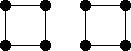
\includegraphics[scale=0.5,frame]{smallGraphs/g_2C4.png}     

\includegraphics[scale=0.5,frame]{smallGraphs/g_2K1.png}     

\includegraphics[scale=0.5,frame]{smallGraphs/g_2K2.png}     
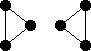
\includegraphics[scale=0.5,frame]{smallGraphs/g_2K3.png}     
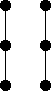
\includegraphics[scale=0.5,frame]{smallGraphs/g_2P3.png}     

\includegraphics[scale=0.5,frame]{smallGraphs/g_3K1.png}     
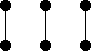
\includegraphics[scale=0.5,frame]{smallGraphs/g_3K2.png}     

\includegraphics[scale=0.5,frame]{smallGraphs/g_4K1.png}     
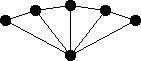
\includegraphics[scale=0.5,frame]{smallGraphs/g_4fan.png}     

\includegraphics[scale=0.5,frame]{smallGraphs/g_5K1.png}     
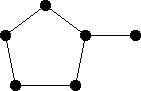
\includegraphics[scale=0.5,frame]{smallGraphs/g_5pan.png}     
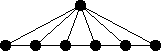
\includegraphics[scale=0.5,frame]{smallGraphs/g_6fan.png}     
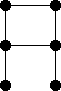
\includegraphics[scale=0.5,frame]{smallGraphs/g_A.png}     
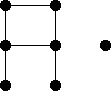
\includegraphics[scale=0.5,frame]{smallGraphs/g_AUK1.png}     
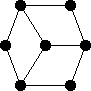
\includegraphics[scale=0.5,frame]{smallGraphs/g_BW3.png}     
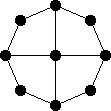
\includegraphics[scale=0.5,frame]{smallGraphs/g_BW4.png}     

\includegraphics[scale=0.5,frame]{smallGraphs/g_C4.png}     

\includegraphics[scale=0.5,frame]{smallGraphs/g_C4U2K1.png}     
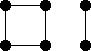
\includegraphics[scale=0.5,frame]{smallGraphs/g_C4UP2.png}     
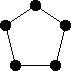
\includegraphics[scale=0.5,frame]{smallGraphs/g_C5.png}     
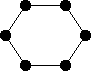
\includegraphics[scale=0.5,frame]{smallGraphs/g_C6.png}     
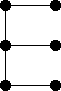
\includegraphics[scale=0.5,frame]{smallGraphs/g_E.png}     
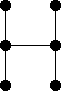
\includegraphics[scale=0.5,frame]{smallGraphs/g_H.png}     
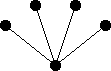
\includegraphics[scale=0.5,frame]{smallGraphs/g_K14.png}     

\includegraphics[scale=0.5,frame]{smallGraphs/g_K2.png}     
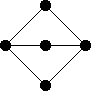
\includegraphics[scale=0.5,frame]{smallGraphs/g_K23.png}     
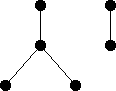
\includegraphics[scale=0.5,frame]{smallGraphs/g_K2Uclaw.png}     
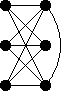
\includegraphics[scale=0.5,frame]{smallGraphs/g_K33+e.png}     
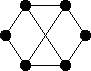
\includegraphics[scale=0.5,frame]{smallGraphs/g_K33-e.png}     
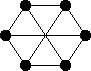
\includegraphics[scale=0.5,frame]{smallGraphs/g_K33.png}     
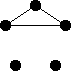
\includegraphics[scale=0.5,frame]{smallGraphs/g_K3U2K1.png}     
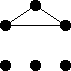
\includegraphics[scale=0.5,frame]{smallGraphs/g_K3U3K1.png}     
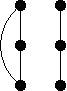
\includegraphics[scale=0.5,frame]{smallGraphs/g_K3UP3.png}     
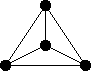
\includegraphics[scale=0.5,frame]{smallGraphs/g_K4.png}     
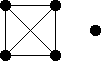
\includegraphics[scale=0.5,frame]{smallGraphs/g_K4UK1.png}     
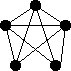
\includegraphics[scale=0.5,frame]{smallGraphs/g_K5-e.png}     
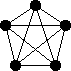
\includegraphics[scale=0.5,frame]{smallGraphs/g_K5.png}     
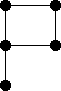
\includegraphics[scale=0.5,frame]{smallGraphs/g_P.png}     

\includegraphics[scale=0.5,frame]{smallGraphs/g_P2UP3.png}     

\includegraphics[scale=0.5,frame]{smallGraphs/g_P2UP4.png}     

\includegraphics[scale=0.5,frame]{smallGraphs/g_P3.png}     

\includegraphics[scale=0.5,frame]{smallGraphs/g_P3U2K1.png}     

\includegraphics[scale=0.5,frame]{smallGraphs/g_P3UP4.png}     

\includegraphics[scale=0.5,frame]{smallGraphs/g_P4.png}     

\includegraphics[scale=0.5,frame]{smallGraphs/g_P5.png}     

\includegraphics[scale=0.5,frame]{smallGraphs/g_P6.png}     
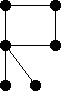
\includegraphics[scale=0.5,frame]{smallGraphs/g_R.png}     
\includegraphics[scale=0.5,frame]{smallGraphs/g_S3.png}     
\includegraphics[scale=0.5,frame]{smallGraphs/g_S4.png}     
\includegraphics[scale=0.5,frame]{smallGraphs/g_T3.png}     
\includegraphics[scale=0.5,frame]{smallGraphs/g_W4.png}     
\includegraphics[scale=0.5,frame]{smallGraphs/g_W4UK1.png}     
\includegraphics[scale=0.5,frame]{smallGraphs/g_W5.png}     
\includegraphics[scale=0.5,frame]{smallGraphs/g_W6.png}     
\includegraphics[scale=0.5,frame]{smallGraphs/g_X1.png}     
\includegraphics[scale=0.5,frame]{smallGraphs/g_X10.png}     
\includegraphics[scale=0.5,frame]{smallGraphs/g_X100.png}     
\includegraphics[scale=0.5,frame]{smallGraphs/g_X101.png}     
\includegraphics[scale=0.5,frame]{smallGraphs/g_X102.png}     
\includegraphics[scale=0.5,frame]{smallGraphs/g_X103.png}     
\includegraphics[scale=0.5,frame]{smallGraphs/g_X104.png}     
\includegraphics[scale=0.5,frame]{smallGraphs/g_X105.png}     
\includegraphics[scale=0.5,frame]{smallGraphs/g_X106.png}     
\includegraphics[scale=0.5,frame]{smallGraphs/g_X107.png}     
\includegraphics[scale=0.5,frame]{smallGraphs/g_X11.png}     
\includegraphics[scale=0.5,frame]{smallGraphs/g_X111.png}     
\includegraphics[scale=0.5,frame]{smallGraphs/g_X12.png}     
\includegraphics[scale=0.5,frame]{smallGraphs/g_X120.png}     
\includegraphics[scale=0.5,frame]{smallGraphs/g_X127.png}     
\includegraphics[scale=0.5,frame]{smallGraphs/g_X13.png}     
\includegraphics[scale=0.5,frame]{smallGraphs/g_X130.png}     
\includegraphics[scale=0.5,frame]{smallGraphs/g_X131.png}     
\includegraphics[scale=0.5,frame]{smallGraphs/g_X132.png}     
\includegraphics[scale=0.5,frame]{smallGraphs/g_X139.png}     
\includegraphics[scale=0.5,frame]{smallGraphs/g_X14.png}     
\includegraphics[scale=0.5,frame]{smallGraphs/g_X140.png}     
\includegraphics[scale=0.5,frame]{smallGraphs/g_X141.png}     
\includegraphics[scale=0.5,frame]{smallGraphs/g_X143.png}     
\includegraphics[scale=0.5,frame]{smallGraphs/g_X146.png}     
\includegraphics[scale=0.5,frame]{smallGraphs/g_X15.png}     
\includegraphics[scale=0.5,frame]{smallGraphs/g_X151.png}     
\includegraphics[scale=0.5,frame]{smallGraphs/g_X153.png}     
\includegraphics[scale=0.5,frame]{smallGraphs/g_X154.png}     
\includegraphics[scale=0.5,frame]{smallGraphs/g_X155.png}     
\includegraphics[scale=0.5,frame]{smallGraphs/g_X158.png}     
\includegraphics[scale=0.5,frame]{smallGraphs/g_X159.png}     
\includegraphics[scale=0.5,frame]{smallGraphs/g_X166.png}     
\includegraphics[scale=0.5,frame]{smallGraphs/g_X167.png}     
\includegraphics[scale=0.5,frame]{smallGraphs/g_X168.png}     
\includegraphics[scale=0.5,frame]{smallGraphs/g_X169.png}     
\includegraphics[scale=0.5,frame]{smallGraphs/g_X17.png}     
\includegraphics[scale=0.5,frame]{smallGraphs/g_X170.png}     
\includegraphics[scale=0.5,frame]{smallGraphs/g_X171.png}     
\includegraphics[scale=0.5,frame]{smallGraphs/g_X172.png}     
\includegraphics[scale=0.5,frame]{smallGraphs/g_X173.png}     
\includegraphics[scale=0.5,frame]{smallGraphs/g_X175.png}     
\includegraphics[scale=0.5,frame]{smallGraphs/g_X176.png}     
\includegraphics[scale=0.5,frame]{smallGraphs/g_X177.png}     
\includegraphics[scale=0.5,frame]{smallGraphs/g_X179.png}     
\includegraphics[scale=0.5,frame]{smallGraphs/g_X18.png}     
\includegraphics[scale=0.5,frame]{smallGraphs/g_X184.png}     
\includegraphics[scale=0.5,frame]{smallGraphs/g_X186.png}     
\includegraphics[scale=0.5,frame]{smallGraphs/g_X195.png}     
\includegraphics[scale=0.5,frame]{smallGraphs/g_X197.png}     
\includegraphics[scale=0.5,frame]{smallGraphs/g_X198.png}     
\includegraphics[scale=0.5,frame]{smallGraphs/g_X199.png}     
\includegraphics[scale=0.5,frame]{smallGraphs/g_X20.png}     
\includegraphics[scale=0.5,frame]{smallGraphs/g_X200.png}     
\includegraphics[scale=0.5,frame]{smallGraphs/g_X205.png}     
\includegraphics[scale=0.5,frame]{smallGraphs/g_X208.png}     
\includegraphics[scale=0.5,frame]{smallGraphs/g_X209.png}     
\includegraphics[scale=0.5,frame]{smallGraphs/g_X21.png}     
\includegraphics[scale=0.5,frame]{smallGraphs/g_X213.png}     
\includegraphics[scale=0.5,frame]{smallGraphs/g_X214.png}     
\includegraphics[scale=0.5,frame]{smallGraphs/g_X23.png}     
\includegraphics[scale=0.5,frame]{smallGraphs/g_X24.png}     
\includegraphics[scale=0.5,frame]{smallGraphs/g_X27.png}     
\includegraphics[scale=0.5,frame]{smallGraphs/g_X29.png}     
\includegraphics[scale=0.5,frame]{smallGraphs/g_X3.png}     
\includegraphics[scale=0.5,frame]{smallGraphs/g_X30.png}     
\includegraphics[scale=0.5,frame]{smallGraphs/g_X31.png}     
\includegraphics[scale=0.5,frame]{smallGraphs/g_X32.png}     
\includegraphics[scale=0.5,frame]{smallGraphs/g_X33.png}     
\includegraphics[scale=0.5,frame]{smallGraphs/g_X34.png}     
\includegraphics[scale=0.5,frame]{smallGraphs/g_X36.png}     
\includegraphics[scale=0.5,frame]{smallGraphs/g_X37.png}     
\includegraphics[scale=0.5,frame]{smallGraphs/g_X38.png}     
\includegraphics[scale=0.5,frame]{smallGraphs/g_X39.png}     
\includegraphics[scale=0.5,frame]{smallGraphs/g_X40.png}     
\includegraphics[scale=0.5,frame]{smallGraphs/g_X42.png}     
\includegraphics[scale=0.5,frame]{smallGraphs/g_X45.png}     
\includegraphics[scale=0.5,frame]{smallGraphs/g_X46.png}     
\includegraphics[scale=0.5,frame]{smallGraphs/g_X5.png}     
\includegraphics[scale=0.5,frame]{smallGraphs/g_X50.png}     
\includegraphics[scale=0.5,frame]{smallGraphs/g_X51.png}     
\includegraphics[scale=0.5,frame]{smallGraphs/g_X58.png}     
\includegraphics[scale=0.5,frame]{smallGraphs/g_X59.png}     
\includegraphics[scale=0.5,frame]{smallGraphs/g_X7.png}     
\includegraphics[scale=0.5,frame]{smallGraphs/g_X71.png}     
\includegraphics[scale=0.5,frame]{smallGraphs/g_X74.png}     
\includegraphics[scale=0.5,frame]{smallGraphs/g_X75.png}     
\includegraphics[scale=0.5,frame]{smallGraphs/g_X79.png}     
\includegraphics[scale=0.5,frame]{smallGraphs/g_X82.png}     
\includegraphics[scale=0.5,frame]{smallGraphs/g_X84.png}     
\includegraphics[scale=0.5,frame]{smallGraphs/g_X85.png}     
\includegraphics[scale=0.5,frame]{smallGraphs/g_X86.png}     
\includegraphics[scale=0.5,frame]{smallGraphs/g_X87.png}     
\includegraphics[scale=0.5,frame]{smallGraphs/g_X88.png}     
\includegraphics[scale=0.5,frame]{smallGraphs/g_X89.png}     
\includegraphics[scale=0.5,frame]{smallGraphs/g_X9.png}     
\includegraphics[scale=0.5,frame]{smallGraphs/g_X90.png}     
\includegraphics[scale=0.5,frame]{smallGraphs/g_X92.png}     
\includegraphics[scale=0.5,frame]{smallGraphs/g_X93.png}     
\includegraphics[scale=0.5,frame]{smallGraphs/g_X95.png}     
\includegraphics[scale=0.5,frame]{smallGraphs/g_X97.png}     
\includegraphics[scale=0.5,frame]{smallGraphs/g_X98.png}     
\includegraphics[scale=0.5,frame]{smallGraphs/g_X99.png}     
\includegraphics[scale=0.5,frame]{smallGraphs/g_XC2.png}     
\includegraphics[scale=0.5,frame]{smallGraphs/g_XC3.png}     
\includegraphics[scale=0.5,frame]{smallGraphs/g_XC5.png}     
\includegraphics[scale=0.5,frame]{smallGraphs/g_XC6.png}     
\includegraphics[scale=0.5,frame]{smallGraphs/g_XC8.png}     
\includegraphics[scale=0.5,frame]{smallGraphs/g_XC9.png}     
\includegraphics[scale=0.5,frame]{smallGraphs/g_XZ11.png}     
\includegraphics[scale=0.5,frame]{smallGraphs/g_XZ13.png}     
\includegraphics[scale=0.5,frame]{smallGraphs/g_XZ14.png}     
\includegraphics[scale=0.5,frame]{smallGraphs/g_antenna.png}     
\includegraphics[scale=0.5,frame]{smallGraphs/g_bull.png}     
\includegraphics[scale=0.5,frame]{smallGraphs/g_butterfly.png}     
\includegraphics[scale=0.5,frame]{smallGraphs/g_butterflyUK1.png}     
\includegraphics[scale=0.5,frame]{smallGraphs/g_claw.png}     
\includegraphics[scale=0.5,frame]{smallGraphs/g_clawU3K1.png}     
\includegraphics[scale=0.5,frame]{smallGraphs/g_clawUK1.png}     
\includegraphics[scale=0.5,frame]{smallGraphs/g_co-2P3.png}     
\includegraphics[scale=0.5,frame]{smallGraphs/g_co-3K2.png}     
\includegraphics[scale=0.5,frame]{smallGraphs/g_co-4fan.png}     
\includegraphics[scale=0.5,frame]{smallGraphs/g_co-5pan.png}     
\includegraphics[scale=0.5,frame]{smallGraphs/g_co-6fan.png}     
\includegraphics[scale=0.5,frame]{smallGraphs/g_co-A.png}     
\includegraphics[scale=0.5,frame]{smallGraphs/g_co-BW3.png}     
\includegraphics[scale=0.5,frame]{smallGraphs/g_co-BW4.png}     
\includegraphics[scale=0.5,frame]{smallGraphs/g_co-C4U2K1.png}     
\includegraphics[scale=0.5,frame]{smallGraphs/g_co-C4UP2.png}     
\includegraphics[scale=0.5,frame]{smallGraphs/g_co-C6.png}     
\includegraphics[scale=0.5,frame]{smallGraphs/g_co-E.png}     
\includegraphics[scale=0.5,frame]{smallGraphs/g_co-H.png}     
\includegraphics[scale=0.5,frame]{smallGraphs/g_co-K23.png}     
\includegraphics[scale=0.5,frame]{smallGraphs/g_co-K2Uclaw.png}     
\includegraphics[scale=0.5,frame]{smallGraphs/g_co-K33-e.png}     
\includegraphics[scale=0.5,frame]{smallGraphs/g_co-K3U2K1.png}     
\includegraphics[scale=0.5,frame]{smallGraphs/g_co-K3U3K1.png}     
\includegraphics[scale=0.5,frame]{smallGraphs/g_co-K5-e.png}     
\includegraphics[scale=0.5,frame]{smallGraphs/g_co-P.png}     
\includegraphics[scale=0.5,frame]{smallGraphs/g_co-P2UP3.png}     
\includegraphics[scale=0.5,frame]{smallGraphs/g_co-P2UP4.png}     
\includegraphics[scale=0.5,frame]{smallGraphs/g_co-P3.png}     
\includegraphics[scale=0.5,frame]{smallGraphs/g_co-P3U2K1.png}     
\includegraphics[scale=0.5,frame]{smallGraphs/g_co-P3UP4.png}     
\includegraphics[scale=0.5,frame]{smallGraphs/g_co-P6.png}     
\includegraphics[scale=0.5,frame]{smallGraphs/g_co-P7.png}     
\includegraphics[scale=0.5,frame]{smallGraphs/g_co-R.png}     
\includegraphics[scale=0.5,frame]{smallGraphs/g_co-W4.png}     
\includegraphics[scale=0.5,frame]{smallGraphs/g_co-W4UK1.png}     
\includegraphics[scale=0.5,frame]{smallGraphs/g_co-W5.png}     
\includegraphics[scale=0.5,frame]{smallGraphs/g_co-W6.png}     
\includegraphics[scale=0.5,frame]{smallGraphs/g_co-X1.png}     
\includegraphics[scale=0.5,frame]{smallGraphs/g_co-X10.png}     
\includegraphics[scale=0.5,frame]{smallGraphs/g_co-X100.png}     
\includegraphics[scale=0.5,frame]{smallGraphs/g_co-X101.png}     
\includegraphics[scale=0.5,frame]{smallGraphs/g_co-X102.png}     
\includegraphics[scale=0.5,frame]{smallGraphs/g_co-X103.png}     
\includegraphics[scale=0.5,frame]{smallGraphs/g_co-X104.png}     
\includegraphics[scale=0.5,frame]{smallGraphs/g_co-X105.png}     
\includegraphics[scale=0.5,frame]{smallGraphs/g_co-X106.png}     
\includegraphics[scale=0.5,frame]{smallGraphs/g_co-X107.png}     
\includegraphics[scale=0.5,frame]{smallGraphs/g_co-X111.png}     
\includegraphics[scale=0.5,frame]{smallGraphs/g_co-X115.png}     
\includegraphics[scale=0.5,frame]{smallGraphs/g_co-X117.png}     
\includegraphics[scale=0.5,frame]{smallGraphs/g_co-X12.png}     
\includegraphics[scale=0.5,frame]{smallGraphs/g_co-X120.png}     
\includegraphics[scale=0.5,frame]{smallGraphs/g_co-X126.png}     
\includegraphics[scale=0.5,frame]{smallGraphs/g_co-X127.png}     
\includegraphics[scale=0.5,frame]{smallGraphs/g_co-X128.png}     
\includegraphics[scale=0.5,frame]{smallGraphs/g_co-X129.png}     
\includegraphics[scale=0.5,frame]{smallGraphs/g_co-X13.png}     
\includegraphics[scale=0.5,frame]{smallGraphs/g_co-X130.png}     
\includegraphics[scale=0.5,frame]{smallGraphs/g_co-X132.png}     
\includegraphics[scale=0.5,frame]{smallGraphs/g_co-X139.png}     
\includegraphics[scale=0.5,frame]{smallGraphs/g_co-X14.png}     
\includegraphics[scale=0.5,frame]{smallGraphs/g_co-X140.png}     
\includegraphics[scale=0.5,frame]{smallGraphs/g_co-X141.png}     
\includegraphics[scale=0.5,frame]{smallGraphs/g_co-X142.png}     
\includegraphics[scale=0.5,frame]{smallGraphs/g_co-X146.png}     
\includegraphics[scale=0.5,frame]{smallGraphs/g_co-X15.png}     
\includegraphics[scale=0.5,frame]{smallGraphs/g_co-X151.png}     
\includegraphics[scale=0.5,frame]{smallGraphs/g_co-X155.png}     
\includegraphics[scale=0.5,frame]{smallGraphs/g_co-X158.png}     
\includegraphics[scale=0.5,frame]{smallGraphs/g_co-X159.png}     
\includegraphics[scale=0.5,frame]{smallGraphs/g_co-X163.png}     
\includegraphics[scale=0.5,frame]{smallGraphs/g_co-X164.png}     
\includegraphics[scale=0.5,frame]{smallGraphs/g_co-X166.png}     
\includegraphics[scale=0.5,frame]{smallGraphs/g_co-X167.png}     
\includegraphics[scale=0.5,frame]{smallGraphs/g_co-X169.png}     
\includegraphics[scale=0.5,frame]{smallGraphs/g_co-X17.png}     
\includegraphics[scale=0.5,frame]{smallGraphs/g_co-X170.png}     
\includegraphics[scale=0.5,frame]{smallGraphs/g_co-X171.png}     
\includegraphics[scale=0.5,frame]{smallGraphs/g_co-X172.png}     
\includegraphics[scale=0.5,frame]{smallGraphs/g_co-X173.png}     
\includegraphics[scale=0.5,frame]{smallGraphs/g_co-X175.png}     
\includegraphics[scale=0.5,frame]{smallGraphs/g_co-X176.png}     
\includegraphics[scale=0.5,frame]{smallGraphs/g_co-X177.png}     
\includegraphics[scale=0.5,frame]{smallGraphs/g_co-X179.png}     
\includegraphics[scale=0.5,frame]{smallGraphs/g_co-X18.png}     
\includegraphics[scale=0.5,frame]{smallGraphs/g_co-X184.png}     
\includegraphics[scale=0.5,frame]{smallGraphs/g_co-X191.png}     
\includegraphics[scale=0.5,frame]{smallGraphs/g_co-X192.png}     
\includegraphics[scale=0.5,frame]{smallGraphs/g_co-X194.png}     
\includegraphics[scale=0.5,frame]{smallGraphs/g_co-X195.png}     
\includegraphics[scale=0.5,frame]{smallGraphs/g_co-X197.png}     
\includegraphics[scale=0.5,frame]{smallGraphs/g_co-X198.png}     
\includegraphics[scale=0.5,frame]{smallGraphs/g_co-X199.png}     
\includegraphics[scale=0.5,frame]{smallGraphs/g_co-X20.png}     
\includegraphics[scale=0.5,frame]{smallGraphs/g_co-X205.png}     
\includegraphics[scale=0.5,frame]{smallGraphs/g_co-X209.png}     
\includegraphics[scale=0.5,frame]{smallGraphs/g_co-X23.png}     
\includegraphics[scale=0.5,frame]{smallGraphs/g_co-X24.png}     
\includegraphics[scale=0.5,frame]{smallGraphs/g_co-X27.png}     
\includegraphics[scale=0.5,frame]{smallGraphs/g_co-X29.png}     
\includegraphics[scale=0.5,frame]{smallGraphs/g_co-X3.png}     
\includegraphics[scale=0.5,frame]{smallGraphs/g_co-X30.png}     
\includegraphics[scale=0.5,frame]{smallGraphs/g_co-X31.png}     
\includegraphics[scale=0.5,frame]{smallGraphs/g_co-X32.png}     
\includegraphics[scale=0.5,frame]{smallGraphs/g_co-X33.png}     
\includegraphics[scale=0.5,frame]{smallGraphs/g_co-X34.png}     
\includegraphics[scale=0.5,frame]{smallGraphs/g_co-X37.png}     
\includegraphics[scale=0.5,frame]{smallGraphs/g_co-X38.png}     
\includegraphics[scale=0.5,frame]{smallGraphs/g_co-X39.png}     
\includegraphics[scale=0.5,frame]{smallGraphs/g_co-X40.png}     
\includegraphics[scale=0.5,frame]{smallGraphs/g_co-X41.png}     
\includegraphics[scale=0.5,frame]{smallGraphs/g_co-X43.png}     
\includegraphics[scale=0.5,frame]{smallGraphs/g_co-X45.png}     
\includegraphics[scale=0.5,frame]{smallGraphs/g_co-X46.png}     
\includegraphics[scale=0.5,frame]{smallGraphs/g_co-X47.png}     
\includegraphics[scale=0.5,frame]{smallGraphs/g_co-X5.png}     
\includegraphics[scale=0.5,frame]{smallGraphs/g_co-X50.png}     
\includegraphics[scale=0.5,frame]{smallGraphs/g_co-X52.png}     
\includegraphics[scale=0.5,frame]{smallGraphs/g_co-X58.png}     
\includegraphics[scale=0.5,frame]{smallGraphs/g_co-X6.png}     
\includegraphics[scale=0.5,frame]{smallGraphs/g_co-X7.png}     
\includegraphics[scale=0.5,frame]{smallGraphs/g_co-X70.png}     
\includegraphics[scale=0.5,frame]{smallGraphs/g_co-X74.png}     
\includegraphics[scale=0.5,frame]{smallGraphs/g_co-X79.png}     
\includegraphics[scale=0.5,frame]{smallGraphs/g_co-X8.png}     
\includegraphics[scale=0.5,frame]{smallGraphs/g_co-X82.png}     
\includegraphics[scale=0.5,frame]{smallGraphs/g_co-X84.png}     
\includegraphics[scale=0.5,frame]{smallGraphs/g_co-X85.png}     
\includegraphics[scale=0.5,frame]{smallGraphs/g_co-X86.png}     
\includegraphics[scale=0.5,frame]{smallGraphs/g_co-X87.png}     
\includegraphics[scale=0.5,frame]{smallGraphs/g_co-X88.png}     
\includegraphics[scale=0.5,frame]{smallGraphs/g_co-X89.png}     
\includegraphics[scale=0.5,frame]{smallGraphs/g_co-X9.png}     
\includegraphics[scale=0.5,frame]{smallGraphs/g_co-X90.png}     
\includegraphics[scale=0.5,frame]{smallGraphs/g_co-X92.png}     
\includegraphics[scale=0.5,frame]{smallGraphs/g_co-X93.png}     
\includegraphics[scale=0.5,frame]{smallGraphs/g_co-X95.png}     
\includegraphics[scale=0.5,frame]{smallGraphs/g_co-X96.png}     
\includegraphics[scale=0.5,frame]{smallGraphs/g_co-X97.png}     
\includegraphics[scale=0.5,frame]{smallGraphs/g_co-X98.png}     
\includegraphics[scale=0.5,frame]{smallGraphs/g_co-X99.png}     
\includegraphics[scale=0.5,frame]{smallGraphs/g_co-antenna.png}     
\includegraphics[scale=0.5,frame]{smallGraphs/g_co-butterfly.png}     
\includegraphics[scale=0.5,frame]{smallGraphs/g_co-butterflyUK1.png}     
\includegraphics[scale=0.5,frame]{smallGraphs/g_co-claw.png}     
\includegraphics[scale=0.5,frame]{smallGraphs/g_co-clawU3K1.png}     
\includegraphics[scale=0.5,frame]{smallGraphs/g_co-clawUK1.png}     
\includegraphics[scale=0.5,frame]{smallGraphs/g_co-cricket.png}     
\includegraphics[scale=0.5,frame]{smallGraphs/g_co-cross.png}     
\includegraphics[scale=0.5,frame]{smallGraphs/g_co-dart.png}     
\includegraphics[scale=0.5,frame]{smallGraphs/g_co-diamond.png}     
\includegraphics[scale=0.5,frame]{smallGraphs/g_co-domino.png}     
\includegraphics[scale=0.5,frame]{smallGraphs/g_co-fish.png}     
\includegraphics[scale=0.5,frame]{smallGraphs/g_co-gem.png}     
\includegraphics[scale=0.5,frame]{smallGraphs/g_co-gemUK1.png}     
\includegraphics[scale=0.5,frame]{smallGraphs/g_co-kiteUK1.png}     
\includegraphics[scale=0.5,frame]{smallGraphs/g_co-longhorn.png}     
\includegraphics[scale=0.5,frame]{smallGraphs/g_co-paw.png}     
\includegraphics[scale=0.5,frame]{smallGraphs/g_co-skewstar.png}     
\includegraphics[scale=0.5,frame]{smallGraphs/g_co-twin-house.png}     
\includegraphics[scale=0.5,frame]{smallGraphs/g_co-twinC5.png}     
\includegraphics[scale=0.5,frame]{smallGraphs/g_cricket.png}     
\includegraphics[scale=0.5,frame]{smallGraphs/g_cross.png}     
\includegraphics[scale=0.5,frame]{smallGraphs/g_dart.png}     
\includegraphics[scale=0.5,frame]{smallGraphs/g_diamond.png}     
\includegraphics[scale=0.5,frame]{smallGraphs/g_domino.png}     
\includegraphics[scale=0.5,frame]{smallGraphs/g_fish.png}     
\includegraphics[scale=0.5,frame]{smallGraphs/g_fork.png}     
\includegraphics[scale=0.5,frame]{smallGraphs/g_gem.png}     
\includegraphics[scale=0.5,frame]{smallGraphs/g_gemUK1.png}     
\includegraphics[scale=0.5,frame]{smallGraphs/g_house.png}     
\includegraphics[scale=0.5,frame]{smallGraphs/g_kite.png}     
\includegraphics[scale=0.5,frame]{smallGraphs/g_kiteUK1.png}     
\includegraphics[scale=0.5,frame]{smallGraphs/g_longhorn.png}     
\includegraphics[scale=0.5,frame]{smallGraphs/g_net.png}     
\includegraphics[scale=0.5,frame]{smallGraphs/g_parachute.png}     
\includegraphics[scale=0.5,frame]{smallGraphs/g_parapluie.png}     
\includegraphics[scale=0.5,frame]{smallGraphs/g_paw.png}     
\includegraphics[scale=0.5,frame]{smallGraphs/g_skewstar.png}     
\includegraphics[scale=0.5,frame]{smallGraphs/g_triangle.png}     
\includegraphics[scale=0.5,frame]{smallGraphs/g_twinC5.png}     

\Closesolutionfile{ans} 

\chapter{Solutions}\begin{answer}{1.4}
The logical implication is:

\[
(A_1 \Rightarrow A_2) \land (A_1 \Rightarrow A_3) \Rightarrow (A_2 \Rightarrow A_3)
\]

For \( A_1(d) = 0 \), \( A_2(d) = 1 \), \( A_3(d) = 0 \), this implication is false. Therefore, the reasoning is incorrect.
\end{answer}
\begin{answer}{1.11}

Let us denote: $A$ – Arthur is a knight, $B$ – Bine is a knight, $C$ – Cene is a knight.

The following compound statement holds:

\[
(A \iff \neg C \lor \neg B) \land (B \iff C \land A)
\]

With the help of the truth table, we see that the statement is true only for the set $A = 1$ and $B = C = 0$.
\end{answer}
\begin{answer}{1.12}
Let \( A \) represent "A is a knight", etc. We seek the only solution \( d \) such that the following is true:

\[
A_1 \land B_1 \land C_1 \land D_1
\]

where:
\begin{align*}
A_1 &: A \iff (\neg D \land \neg C)\\
B_1 &: B \iff (\neg A \land \neg D \Rightarrow \neg C)\\
C_1 &: C \iff (\neg B \Rightarrow A)\\
D_1 &: D \iff (\neg E \Rightarrow \neg C \land \neg B)\\
\end{align*}


Since the truth table would contain 32 rows, we solve this by analyzing cases.

\subsection*{Case 1: \( A(d) = 1 \)}

Given \( A_1 \), \( D(d) = 0 \) and \( C(d) = 0 \). Substituting into \( C_1 \) with \( A(d) = 1 \) and \( C(d) = 0 \), we get:

\[
\neg (\neg B \Rightarrow 1) \Rightarrow \neg(B \lor 1) \Rightarrow \neg 1
\]

which is a false statement. Hence, this case is not possible.

\subsection*{Case 2: \( A(d) = 0 \)}

Given \( A_1 \), either \( C(d) = 1 \) or \( D(d) = 1 \).

\subsection*{Case 2.1: \( C(d) = 1 \)}

Since \( C_1 \), \( \neg B \Rightarrow 0 \), implies \( \neg B = 0 \), hence \( B(d) = 1 \).

Substituting into \( B_1 \) with \( A(d) = 0 \), \( B(d) = 1 \), and \( C(d) = 1 \), we get:

\[
1 \land \neg D \Rightarrow 0 \Rightarrow \neg D = 0
\]

thus, \( D(d) = 1 \).

Substituting into \( D_1 \), we get:

\[
\neg E \Rightarrow 0 \land 0
\]

Hence \( E(d) = 1 \).

\subsection*{Case 2.2: \( C(d) = 0 \) and \( D(d) = 1 \)}

From \( B_1 \), we get \( B(d) = 1 \), but the statement \( C_1 \) becomes false: \( 0 \iff (0 \Rightarrow 1) \).

Thus, \( B \), \( C \), \( D \), and \( E \) are knights, while \( A \) is a servant.

\end{answer}
\begin{answer}{1.27}

\begin{eqnarray*}
(A\Rightarrow B) \vee (B \Rightarrow C) &\Leftrightarrow & (\neg A \vee B) \vee (\neg B \vee C)\\
&\Leftrightarrow & \neg A \vee B \vee \neg B \vee C\\
&\Leftrightarrow & \neg A \vee (B \vee \neg B) \vee C\\
&\Leftrightarrow & \neg A \vee 1 \vee C\\
&\Leftrightarrow & 1.
\end{eqnarray*}
\end{answer}
\begin{answer}{1.34}
    We need to show that $x + \frac{1}{x} \geq 2$. Since $x \geq 0$, we can multiply the inequality by $x$ to get
    \[
    x^2 + 1 \geq 2x
    \]
    or equivalently,
    \[
    (x - 1)^2 \geq 0.
    \]
    This is obviously always true.
\end{answer}
\begin{answer}{1.35}
    Suppose there are only finitely many primes $p_1, p_2, \ldots, p_n$. Then the number $p = p_1 p_2 \cdots p_n + 1$ is not divisible by any prime $p_i$ and $p_i \neq p$ for each $i$. By definition, $p$ is therefore a prime number that is different from each of the previous ones. This is a contradiction.
\end{answer}
\begin{answer}{1.36}
    The opposite statement is: there exists a natural number greater than $1$.
\end{answer}
\begin{answer}{1.38}
We prove both directions separately:

($\Rightarrow$) Assume that $m$ and $n$ have different parities. Write $m = 2k$ and $n = 2l + 1$, substitute into the expression $m^2 - n^2$, and the result follows.

    ($\Leftarrow$) We show indirectly: If $m$ and $n$ have the same parity, then $m^2 - n^2$ is even. Consider both cases.
\end{answer}
\begin{answer}{1.40}
    \begin{enumerate}[label=(\roman*)]
        \item $(A \Rightarrow B) \wedge A \Rightarrow B$. This is true.
        \item  $(A \Rightarrow B) \wedge \neg A \Rightarrow \neg B$. This is not necessarily true.
        \item $((A \Rightarrow B) \wedge \neg A) \Rightarrow \neg B$. This is not necessarily true.
        \item $((A \Rightarrow B) \wedge (B \Rightarrow C)) \Rightarrow (\neg C \Rightarrow \neg A)$. This is true.
    \end{enumerate}
\end{answer}
\begin{answer}{2.2}
    \begin{enumerate}[label=(\roman*)]
        \item $P\cap S \neq \emptyset$
        \item $0 \in \mathbb{Z}\setminus \mathbb{N}$
        \item $\mathbb{N}\subseteq \mathbb{Z}$
        \item $\mathbb{Z}\nsubseteq \mathbb{N}$
        \item $P\setminus \{2\} \subseteq \overline{S}$
        \item $2\in S\cap P$
    \end{enumerate}
\end{answer}
\begin{answer}{2.4}
\begin{eqnarray*}
x\in (A\cup C)\cap (B\setminus C) &\Leftrightarrow & (x\in A \vee x\in C) \wedge (x\in B \wedge x\notin C)\\
 &\Leftrightarrow & ((x\in A \vee x\in C) \wedge (x\notin C))\wedge x\notin B\\
&\Leftrightarrow & ((x\in A \wedge x\notin C) \vee (x\in C \wedge x\notin C)) \wedge
 x\in B\\
&\Leftrightarrow & x\in A \wedge x\notin C  \wedge x\in B\\
&\Leftrightarrow & x\in A \wedge x\in B  \wedge x\notin C \\
&\Leftrightarrow & x \in (A\cap B)\setminus C.
\end{eqnarray*}
\end{answer}
\begin{answer}{2.5}
    Use direct proof.
\end{answer}
\begin{answer}{2.6}
    Prove separately each direction.
\end{answer}
\begin{answer}{2.7}

\begin{eqnarray*}
(x,y)\in A\times (B\cap C) &\Leftrightarrow & x \in A \wedge y\in B\cap C\\
&\Leftrightarrow & x \in A \wedge y\in B  \wedge y\in C\\
&\Leftrightarrow & x \in A \wedge x \in A\wedge y\in B  \wedge y\in C\\
&\Leftrightarrow & x \in A \wedge  y\in B  \wedge x \in A\wedge y\in C\\
&\Leftrightarrow & (x,y) \in A\times B \wedge  (x,y) \in A\times C\\
&\Leftrightarrow & (x,y) \in (A\times B)\cap   (A\times C).
\end{eqnarray*}
\end{answer}
\begin{answer}{2.8}

\begin{eqnarray*}
x\in (A\cap B )\setminus B  &\Leftrightarrow & x \in (A\cap B)  \wedge x\notin B\\
&\Leftrightarrow & (x\in A\wedge x\in  B ) \wedge x\notin B\\
&\Leftrightarrow & x\in A\wedge (x\in  B  \wedge x\notin B)\\
&\Leftrightarrow & x\in \emptyset.
\end{eqnarray*}
\end{answer}
\begin{answer}{2.10}
 (In slovene.)

\begin{enumerate}
\item Napačna. Vzemi $A=\emptyset$, $B=\{\emptyset\}$, $B=\{\{\emptyset\}\}$.
\item Napačna. Vzemi isti primer kot v (a).
\item Pravilna. Dokaz s protislovjem. Recimo, da trditev ni pravilna. Naj bo $A\cap B\subseteq \overline{C}$, $A\cup C\subseteq B$  in naj obstaja $x\in A\cap C$. Torej je $x\in A$ in $x\in C$. Ker je po drugi predpostavki $A\cup C\subseteq B$, je $x\in B$. Sledi $x\in A \cap B$. Ker je po prvi predpostavki $A\cap B\subseteq \overline{C}$, je $x\in \overline{C}$. Protislovje, saj $x\in C$.
\item Napačna. Vzemi $A=C\neq B$.
\item Napačna. Vzemi tri paroma disjunktne neprazne množice.
\end{enumerate}

\end{answer}
\begin{answer}{2.21}
    \begin{enumerate}
\item[$\rightarrow$]
Let $A\subseteq B$.
We will show that $A\cap \overline{B} = \emptyset$ holds. By assumption, we have
\begin{equation}\label{eq:4}
(\forall x)(x\in A \Rightarrow x\in B).
\end{equation}
Suppose that there exists $x\in A\cap \overline{B}$. Then
\begin{eqnarray*}
x\in A\cap \overline{B} &\Rightarrow & x\in A \wedge x\in \overline{B}\\
						&\Rightarrow & x\in A \wedge x \notin B\\
						&\Rightarrow & x\in B \wedge x \notin B \quad (\textrm{due to } (\ref{eq:4})),
\end{eqnarray*}
a contradiction. Therefore, $A\cap \overline{B}=\emptyset$.

$\leftarrow$ Let $A\cap \overline{B}=\emptyset$. We will show that $A\subseteq B$. Take any $x\in A$. Then $x\notin \overline{B}$, since $A\cap \overline{B}=\emptyset$. Thus, $x\in B$. Since $x$ was arbitrary, it follows that $A\subseteq B$.

\item
\begin{eqnarray*}
A\setminus B & = & \{x\, ;\, x\in A \wedge x\notin B \}\\
             & = & \{x\, ;\, x\notin \overline{A} \wedge x  \in \overline{B} \}\\
             & = & \{x\, ; x\,  \in \overline{B} \wedge  x\notin \overline{A} \}\\
             & = & \overline{B} \setminus \overline{A}.
\end{eqnarray*}

\end{enumerate}


\end{answer}
\begin{answer}{3.4}
    \begin{enumerate}
    \item Domain: \(\{1, 2, 3\}\), Range: \(\{2, 3, 4\}\)
    \item Domain: \(\{1, 2, 3, 4\}\), Range: \(\{5, 3, 9\}\)
    \item Domain: \(\{1, 3, 4\}\), Range: \(\{2, 5\}\)
    \item Domain: \(\{-1, 2, 3\}\), Range: \(\{-1, 2, 3\}\)
    \item Domain: \(\{2, 9\}\), Range: \(\{0\}\)
\end{enumerate}

\end{answer}
\begin{answer}{3.6}
        For \(R_1 = \{(1, 2), (2, 3), (3, 4)\}\) and \(R_2 = \{(2, 4), (3, 5), (4, 6)\}\):
    \[
    R_2 \circ R_1 = \{(1, 4), (2, 5), (3, 6)\}, \quad R_1 \circ R_2 = \{(2, 4), (3, 5)\}.
    \]
    They are \textbf{not equal} because composition is not commutative.
    
\end{answer}
\begin{answer}{3.7}
    \begin{enumerate}
        \item \(R_2 \circ R_1 = \{(1, 6), (2, 4)\}\)
        \item \(R_2 \circ R_1 = \{(1, 4), (2, 6), (3, 4)\}\)
        \item \(R_2 \circ R_1 = \{(4, 5), (5, 6), (6, 4)\}\)
        \item \(R_1 \circ R_1 = \{(4, 4), (5, 5), (6, 6)\}\)
    \end{enumerate}
\end{answer}
\begin{answer}{3.8}
    \(R_1 = \{(x, y) \mid y = x + 1\}\), \(R_2 = \{(y, z) \mid z = y + 2\}\):
    \[
    R_2 \circ R_1 = \{(x, z) \mid z = x + 3, \, x, z \in \mathbb{Z}\}.
    \]
    
\end{answer}
\begin{answer}{3.9}
        For \(R = \{(1, 2), (2, 3), (3, 4)\}\):
    \[
    R \circ R = \{(1, 3), (2, 4)\}, \quad R \circ R \circ R = \{(1, 4)\},
    \]
    while \(R \circ R \circ R \circ R \circ R=\emptyset\)
    
\end{answer}
\begin{answer}{3.14}
        To check transitivity:
If \((x, y) \in R\) and \((y, z) \in R\), then \((x, z) \in R\).
Here, \((1, 2) \in R\) and \((2, 3) \in R\), but \((1, 3) \notin R\).
Thus, \(R\) is \textbf{not transitive}.

    
\end{answer}
 


\end{document}
